%%%%%%%%%%%%%%%%%%%%%%%%%%%%%%%%%%%%%%%%%%%%%%%%%%%%%%%%%%%%%%%%%%%%%%%%%%%%%%%
% Capitolo: Parte Analogica
%%%%%%%%%%%%%%%%%%%%%%%%%%%%%%%%%%%%%%%%%%%%%%%%%%%%%%%%%%%%%%%%%%%%%%%%%%%%%%%
\chapter{Parte Analogica}

\section{Circuiti Equivalenti e Amplificatori}

%------------------------%
\subsection{Calcolo dei parametri caratteristici del circuito equivalente “rete due porte” di un invertente}

Consideriamo l'operazionale illustrato in Figura~\ref{fig:inverting_amp}.\\[2mm]
\begin{figure}[H]
    \centering
    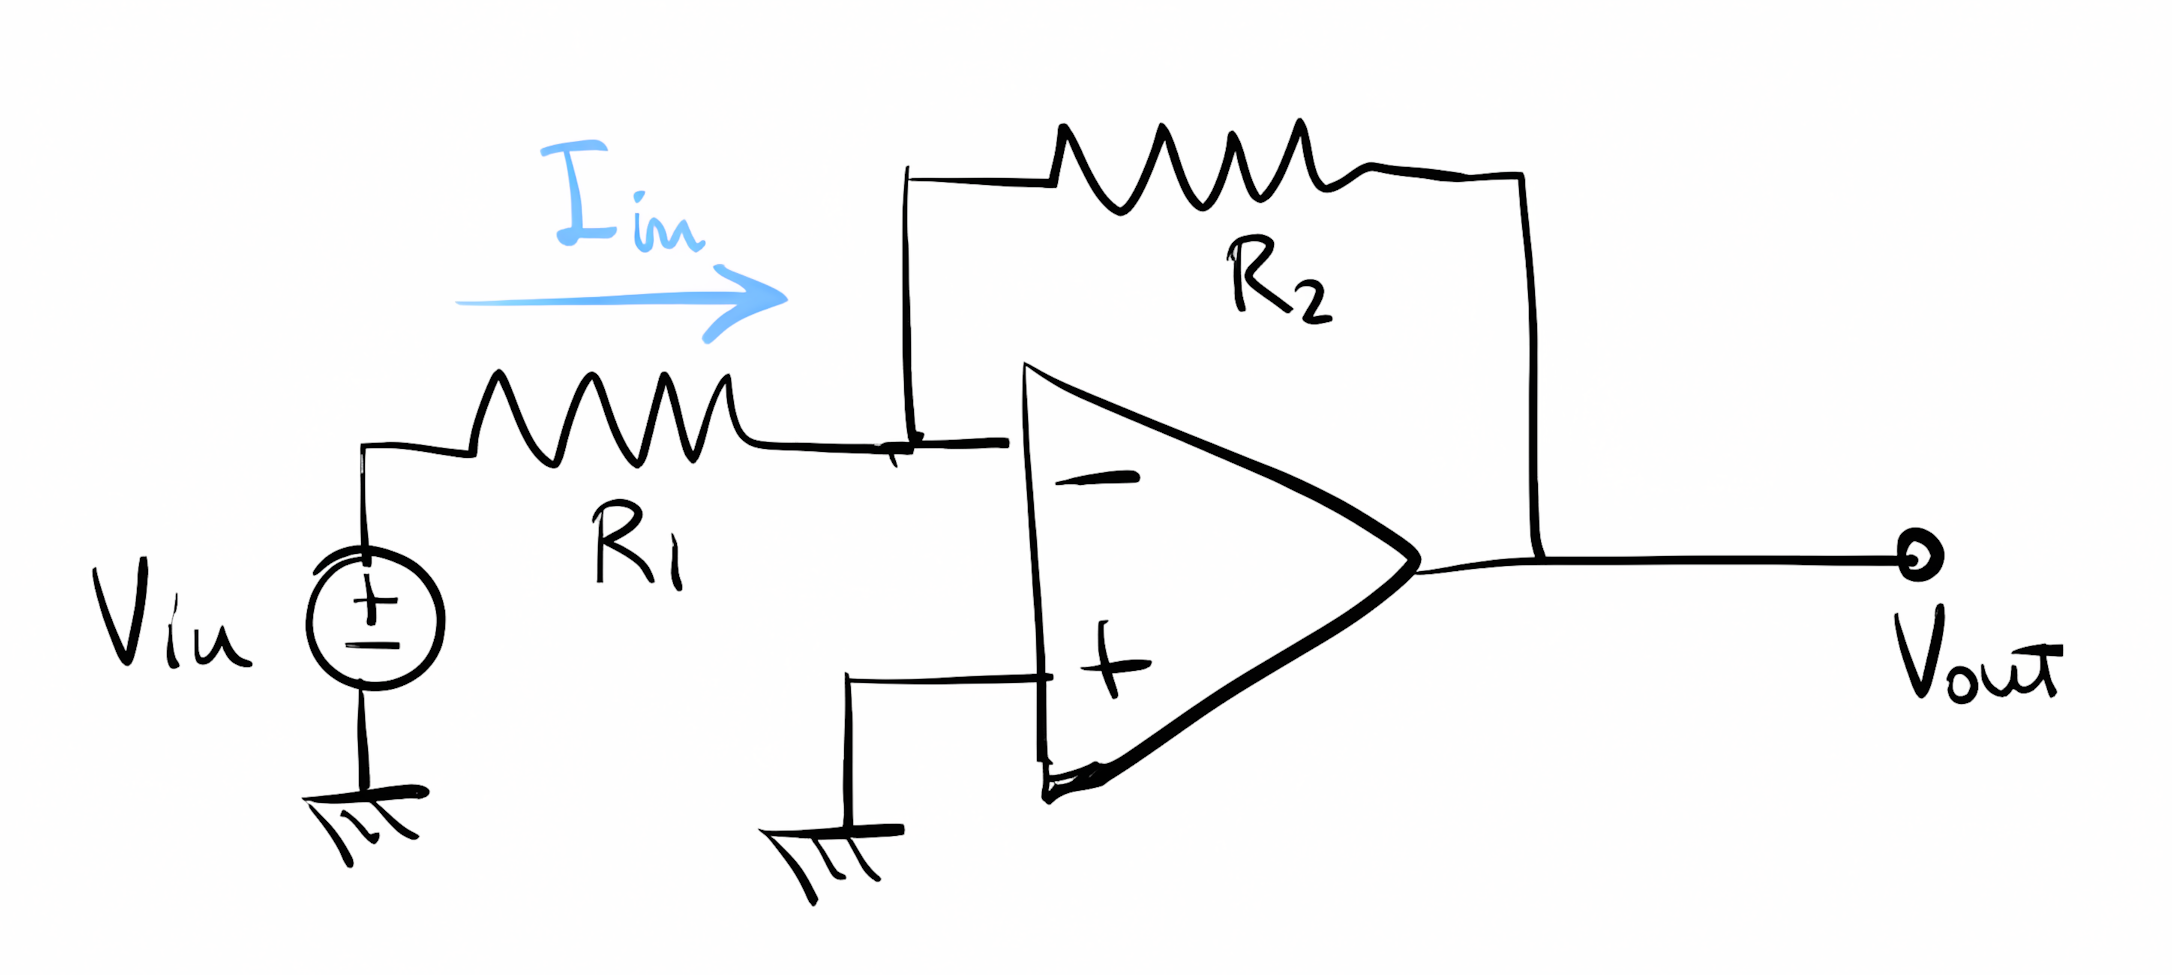
\includegraphics[width=0.6\textwidth]{images/1.1.1.1.png}
    \caption{Amplificatore operazionale in configurazione invertente.}
    \label{fig:inverting_amp}
\end{figure}

L'obiettivo è rappresentare il circuito con un modello equivalente a due porte, come quello studiato a lezione (vedi, ad esempio, Figura~\ref{fig:rete_due_porte_d}).\\[2mm]
\begin{figure}[H]
    \centering
    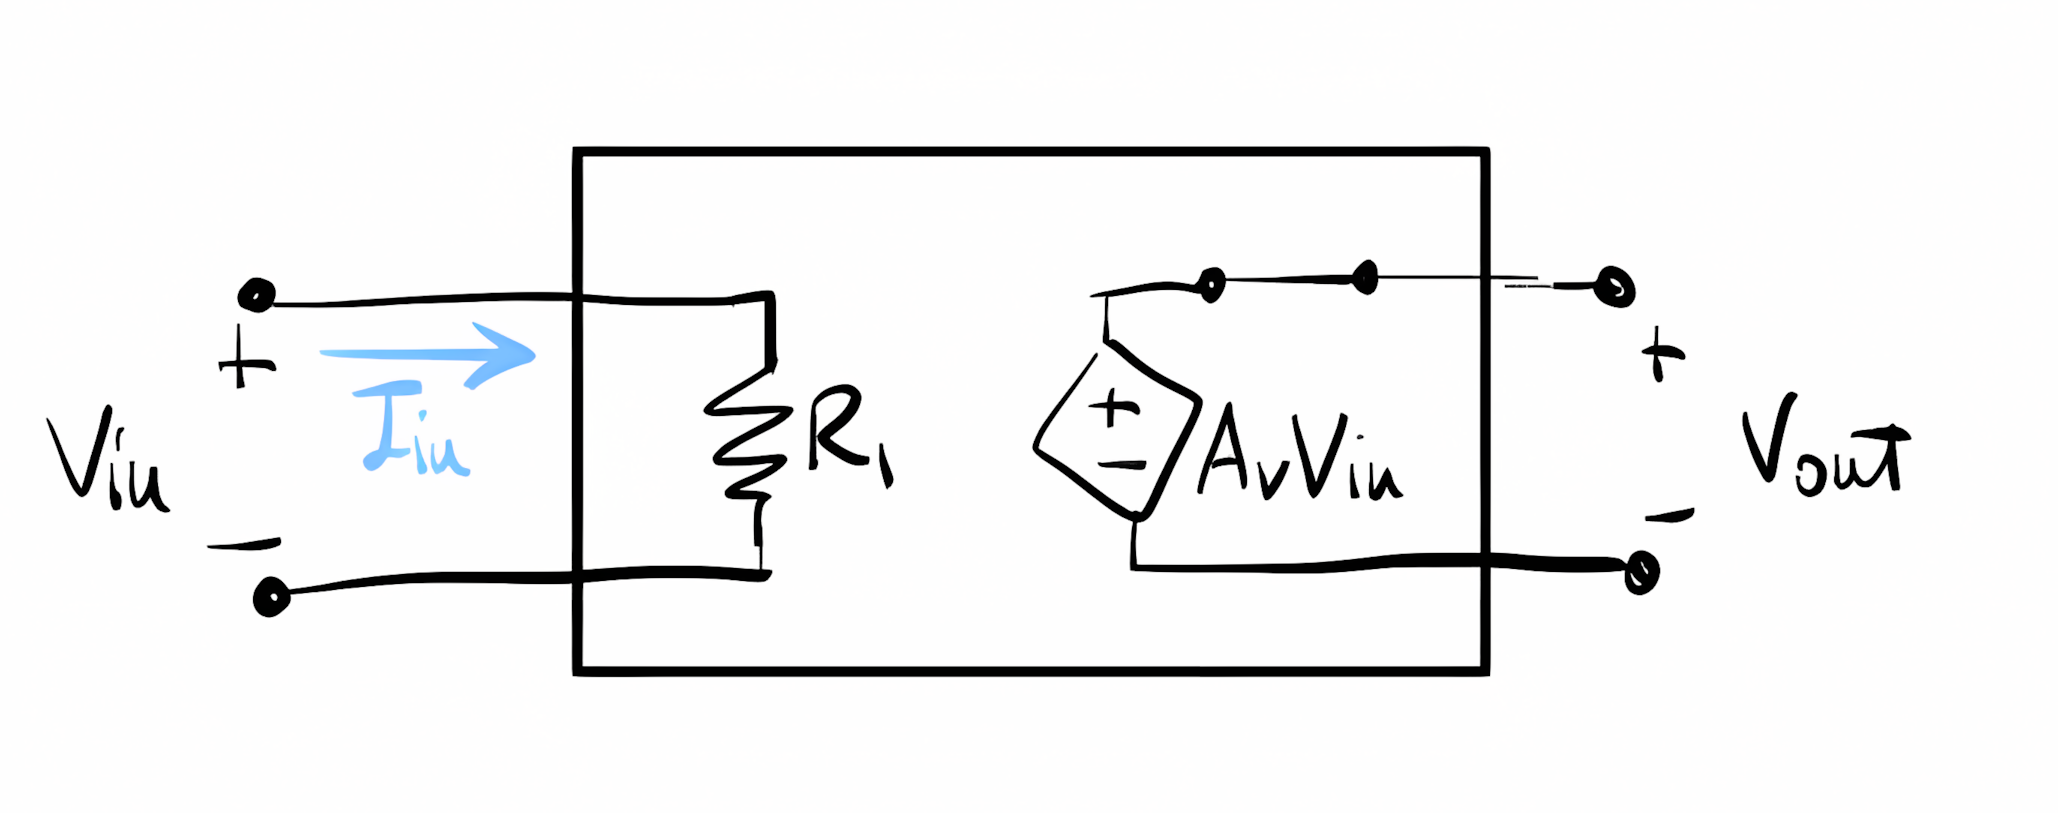
\includegraphics[width=0.6\textwidth]{images/1.1.1.2.png}
    \caption{Circuito a due porte equivalente di una configurazione invertente.}
    \label{fig:rete_due_porte_d}
\end{figure}

Nel caso dell'amplificatore invertente, dalla nota relazione
\[
V_{\text{out}} = -\frac{R_2}{R_1}\, V_{\text{in}},
\]
si deduce immediatamente che:
\[
g_{21} = -\frac{R_2}{R_1} \quad \text{e} \quad g_{22} = 0.
\]
Inoltre, poiché la corrente d’ingresso è data unicamente dalla caduta su \(R_1\),
\[
I_{\text{in}} = \frac{V_{\text{in}}}{R_1},
\]
abbiamo:
\[
g_{11} = \frac{1}{R_1} \quad \text{e} \quad g_{12} = 0.
\]
Verificando la correttezza di tale analisi (ad esempio, sostituendo \(V_{\text{out}}\) con un generatore \(V_x\) e annullando \(V_{\text{in}}\)), la corrente in uscita fluisce direttamente verso massa senza contribuire a \(I_{\text{in}}\).

Il circuito equivalente risultante è mostrato nella medesima Figura~\ref{fig:rete_due_porte_d}.

\newpage

%------------------------%
\subsection{Circuito equivalente “rete due porte” di un transistor MOS per piccoli segnali e definizione di “piccoli segnali”}

Il circuito equivalente “rete due porte” per piccoli segnali è composto da un'impedenza infinita in ingresso (circuito aperto) e da un generatore di corrente \(g_m V_{GS}\), dove \(V_{GS}\) è la differenza di potenziale tra gate e source.

Consideriamo un circuito amplificatore con transistor MOS, avente ingresso \(v_{\text{in}}\) polarizzato da un generatore \(V_P\). La funzione di trasferimento, mostrata in Figura~\ref{fig:mos_equivalente_transf}, presenta una zona centrale (punto di lavoro) in cui la curva risulta approssimabile a una funzione lineare, e quindi il parametro \(G_m\) diventa una costante \(g_m\).\\[2mm]
\begin{figure}[H]
    \centering
    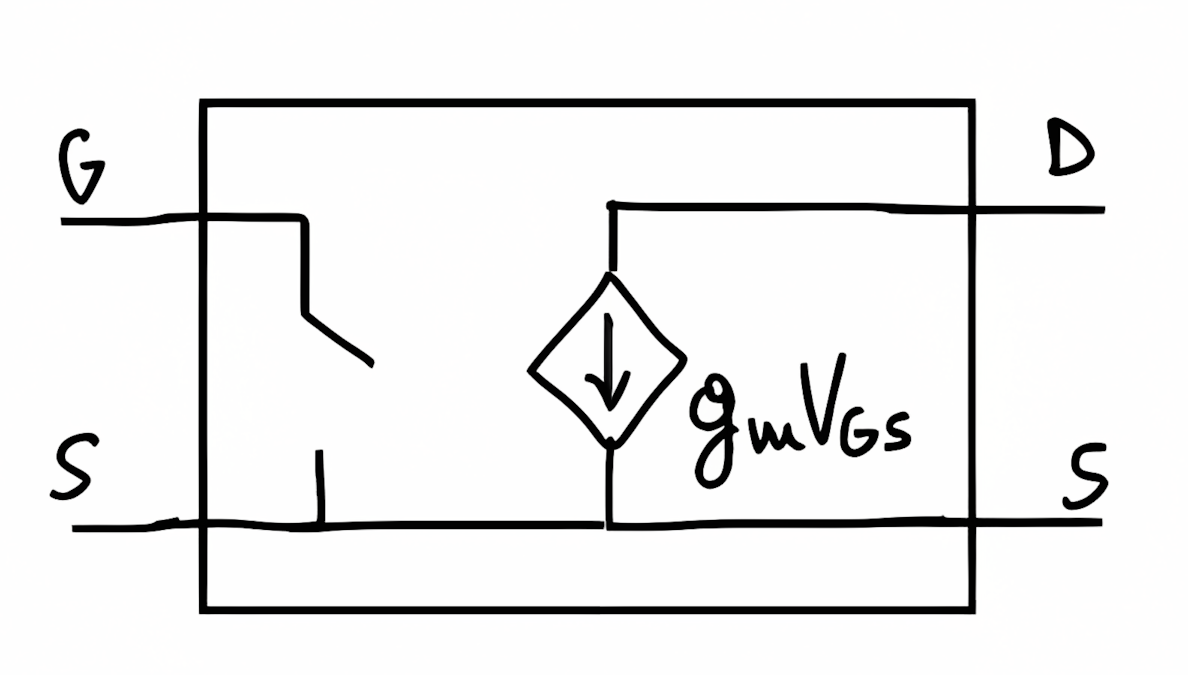
\includegraphics[width=0.6\textwidth]{images/1.1.2.1.png}
    \caption{Circuito equivalente “rete due porte” di un transistor MOS per piccoli segnali.}
    \label{fig:mos_equivalente}
\end{figure}

\begin{figure}[H]
    \centering
    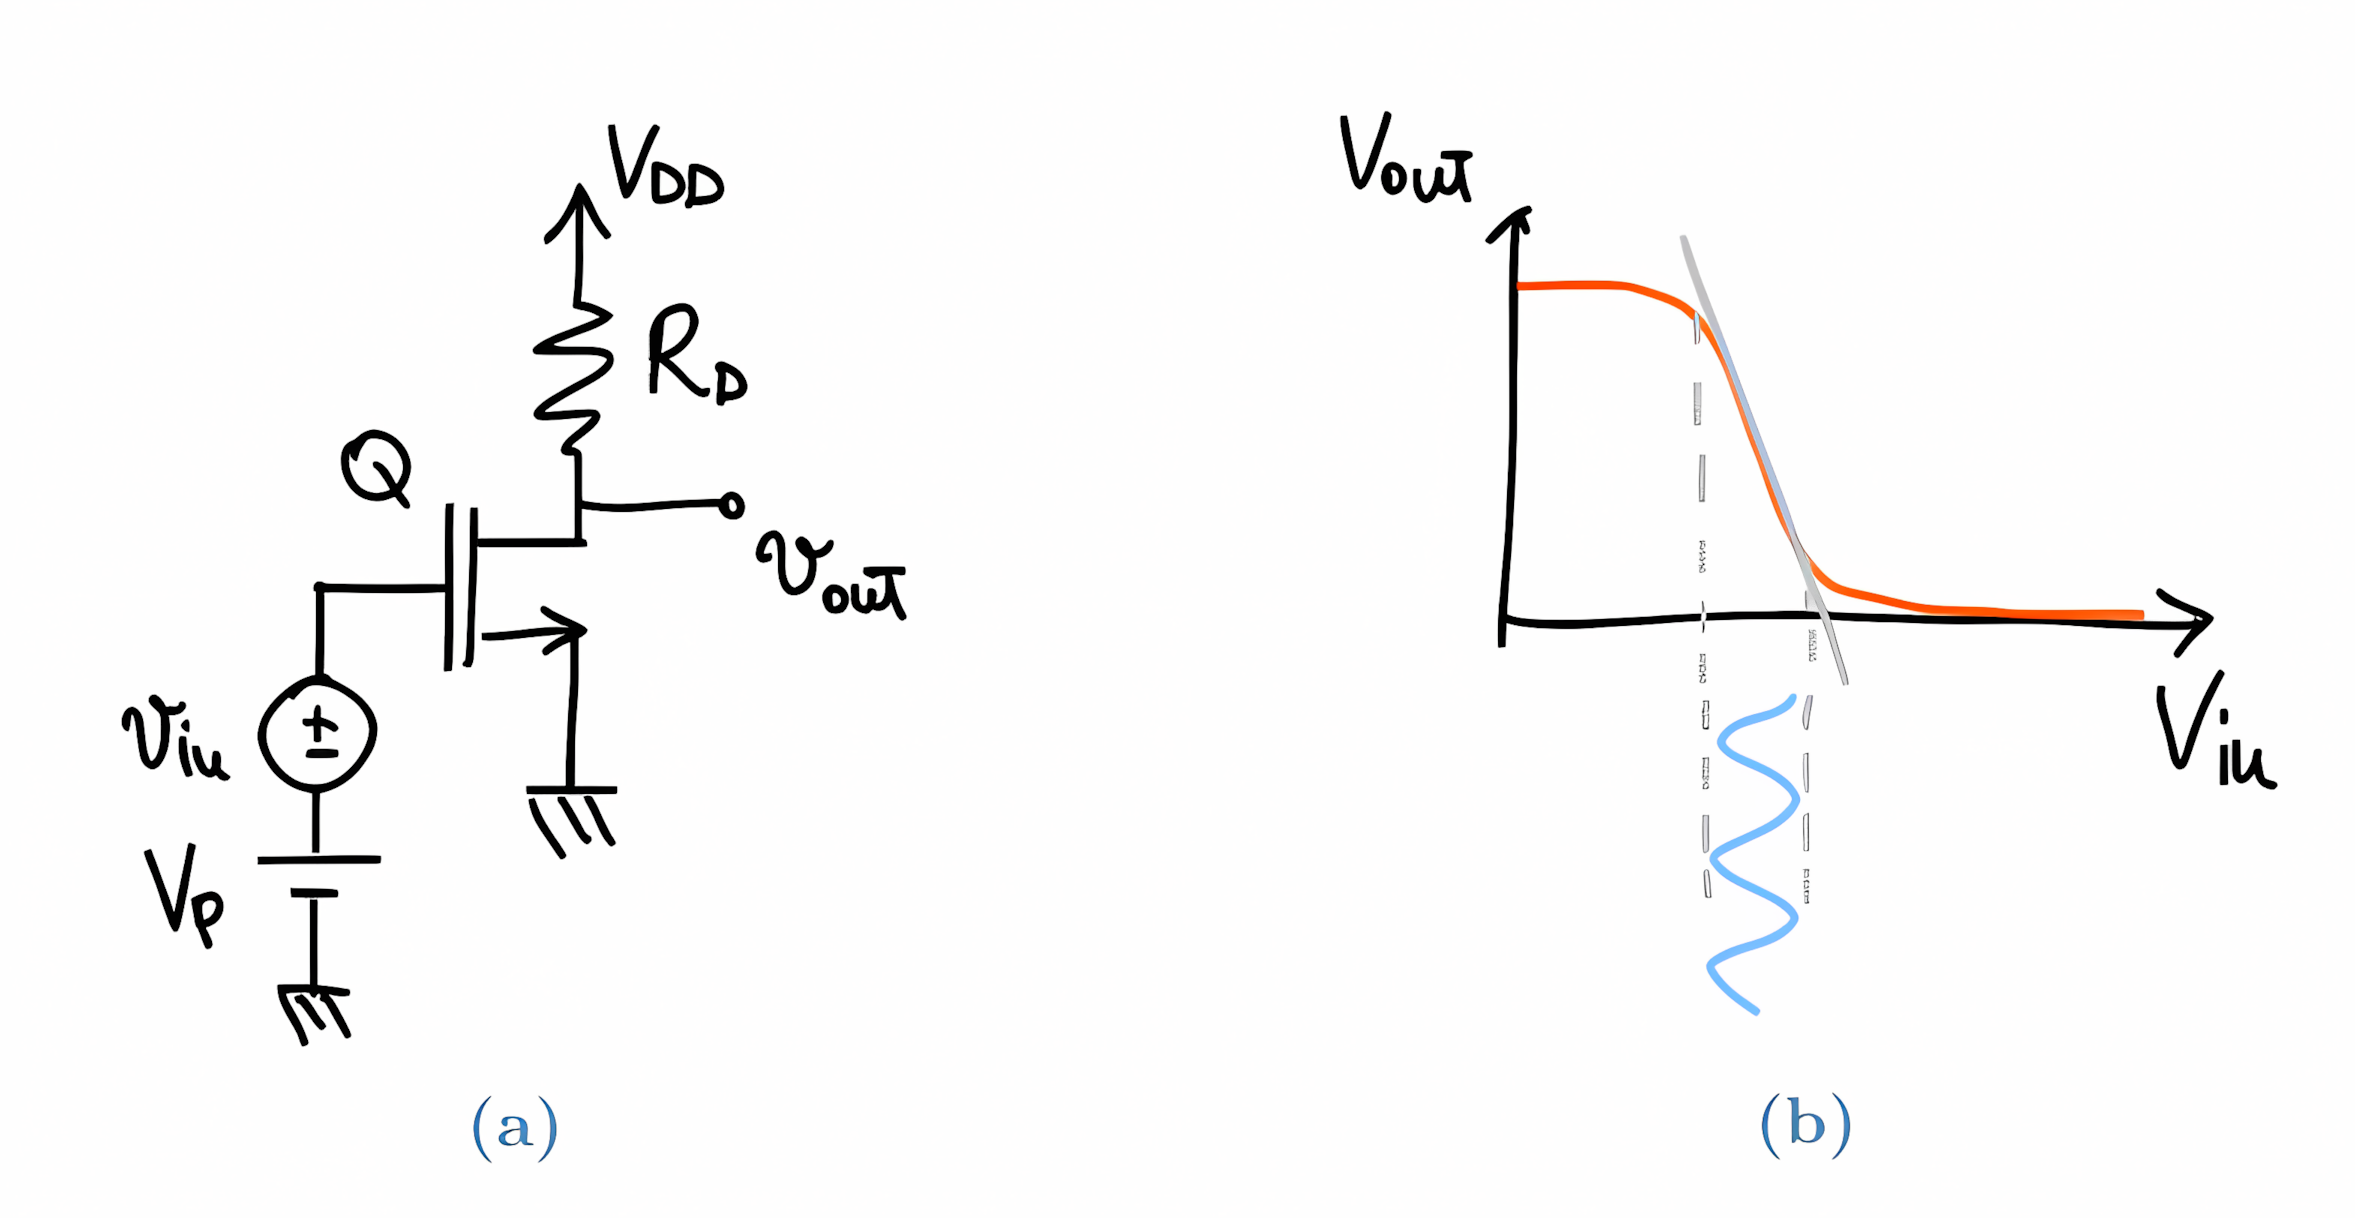
\includegraphics[width=0.6\textwidth]{images/1.1.2.2.png}
    \caption{(a) Circuito amplificatore con MOS, con ingresso \(v_{\text{in}}\) polarizzato da \(V_P\); (b) Trascaratteristica: nel punto di lavoro la risposta è approssimabile a una funzione lineare.}
    \label{fig:mos_equivalente_transf}
\end{figure}

Per analizzare quando tale approssimazione è valida, consideriamo il transistor \(Q\) in saturazione:
\[
i_D = k (V_{GS} - V_t)^2 = k \Bigl(v_{\text{in}} + (V_P - V_t)\Bigr)^2.
\]
Espandendo:
\[
i_D = k \left(v_{\text{in}}^2 + 2(V_P - V_t)v_{\text{in}} + (V_P - V_t)^2\right)
= k\, v_{\text{in}}^2 + 2k(V_P - V_t)v_{\text{in}} + I_P,
\]
dove \(I_P = k (V_P - V_t)^2\) è la corrente di polarizzazione, dovuta esclusivamente a \(V_P\). Affinché la relazione sia linearizzata, il termine \(v_{\text{in}}^2\) deve essere trascurabile:
\[
v_{\text{in}}^2 \ll 2(V_P - V_t)v_{\text{in}} \quad \Longrightarrow \quad v_{\text{in}} \ll 2(V_P - V_t).
\]
Pertanto, il segnale è definito “piccolo” quando \(v_{\text{in}}\) è almeno un ordine di grandezza inferiore a \(2(V_P - V_t)\).

\newpage

%------------------------%
\subsection{Circuiti equivalenti per grandi segnali in continua per i tre casi}

Il segnale in ingresso è la differenza \(V_{GS}\) tra gate e source. In un MOSFET il circuito tra gate e source è in circuito aperto, mentre il comportamento in uscita varia in base ai valori di \(V_{GS}\) e \(V_{DS}\).

Distinguiamo tre casi:
\begin{enumerate}
    \item \textbf{Interdizione}: \(V_{GS} < V_t\). Tra drain e source il MOSFET è in circuito aperto (vedi Figura~\ref{fig:mos_grandi}a).
    \item \textbf{Triodo}: \(V_{GS} > V_t\) e \(V_{DS} < V_{GS} - V_t\). Il dispositivo si comporta come una resistenza variabile (Figura~\ref{fig:mos_grandi}b).
    \item \textbf{Saturazione}: \(V_{GS} > V_t\) e \(V_{DS} > V_{GS} - V_t\). Il dispositivo si comporta come un generatore di corrente controllato, approssimabile con \(g_m V_{GS}\) (Figura~\ref{fig:mos_grandi}c).
\end{enumerate}

\begin{figure}[H]
    \centering
    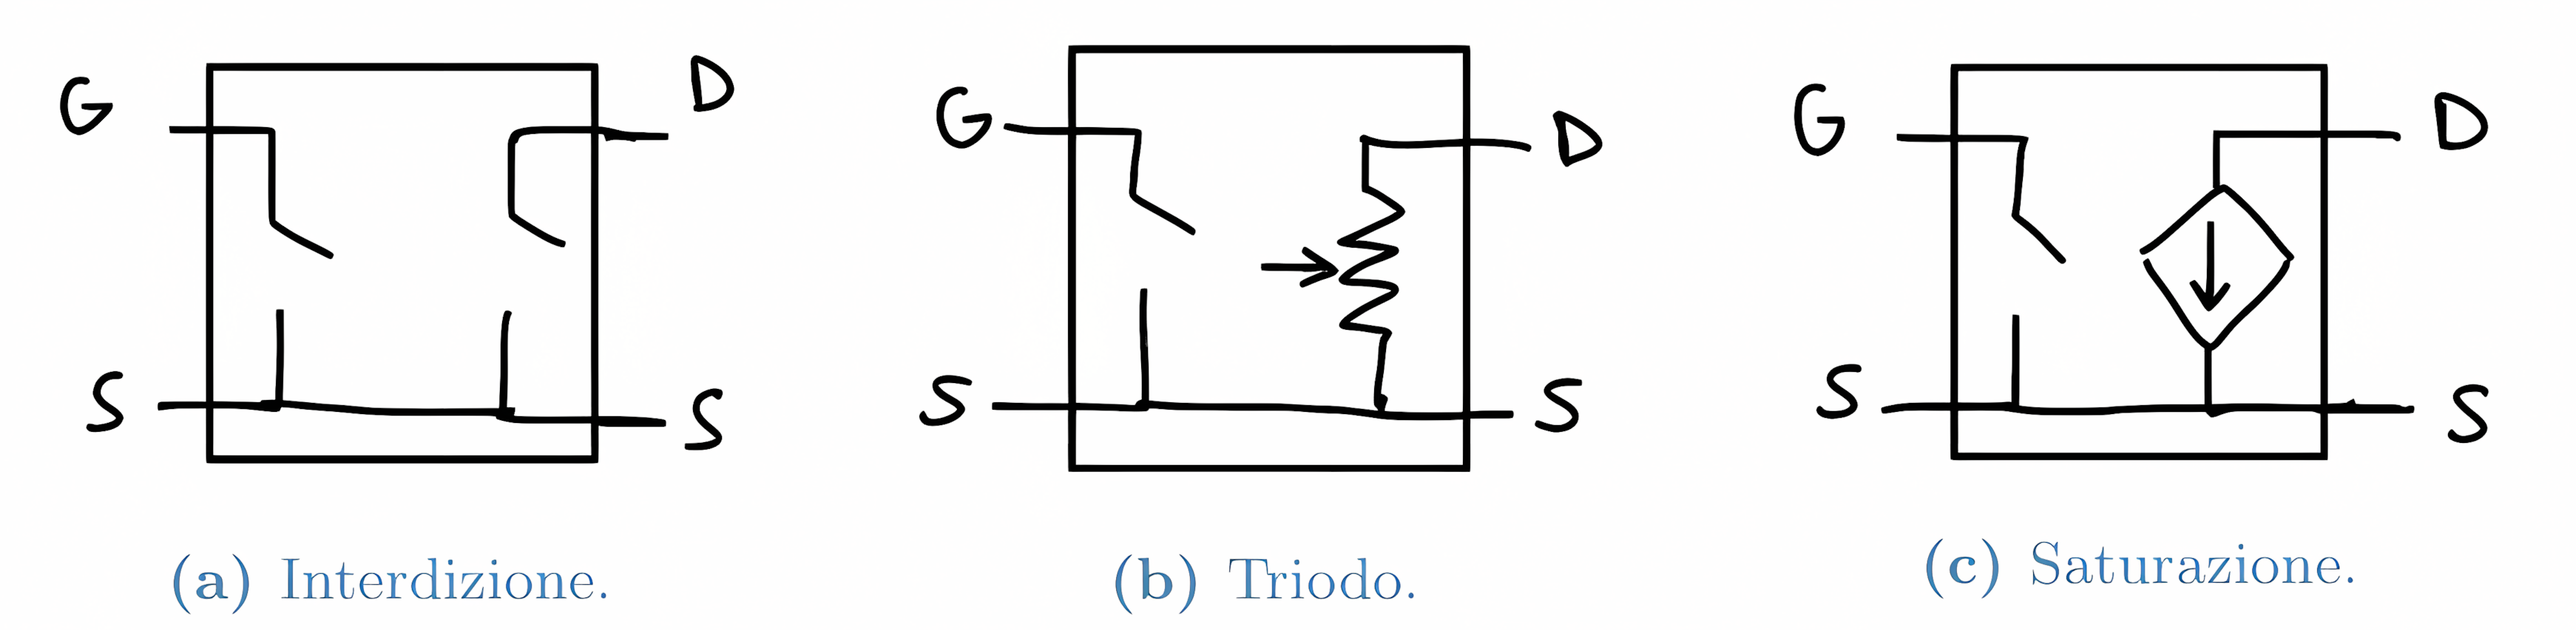
\includegraphics[width=0.8\textwidth]{images/1.1.3.1.png}
    \caption{Circuiti equivalenti di un transistor MOSFET nei tre casi: (a) interdizione, (b) triodo, (c) saturazione.}
    \label{fig:mos_grandi}
\end{figure}

\newpage
%%%%%%%%%%%%%%%%%%%%%%%%%%%%%%%%%%%%%%%%%%%%%%%%%%%%%%%%%%%%%%%%%%%%%%%%%%%%%%%
\section{Amplificatori di Transresistenza e Operazionali}

\subsection{Parametri ideali “rete due porte” di un amplificatore di transresistenza \(V_{\text{out}}/I_{\text{in}}\), confronto tra invertente e non invertente}

L'amplificatore di transresistenza presenta una corrente in ingresso \(I_{\text{in}}\) e una tensione in uscita
\[
V_{\text{out}} = R_m I_{\text{in}},
\]
dove
\[
R_m = \frac{V_{\text{out}}}{I_{\text{in}}} \quad \text{con } I_{\text{out}} = 0.
\]
Lo schema equivalente “rete due porte” è mostrato in Figura~\ref{fig:transresistenza}.\\[2mm]
\begin{figure}[H]
    \centering
    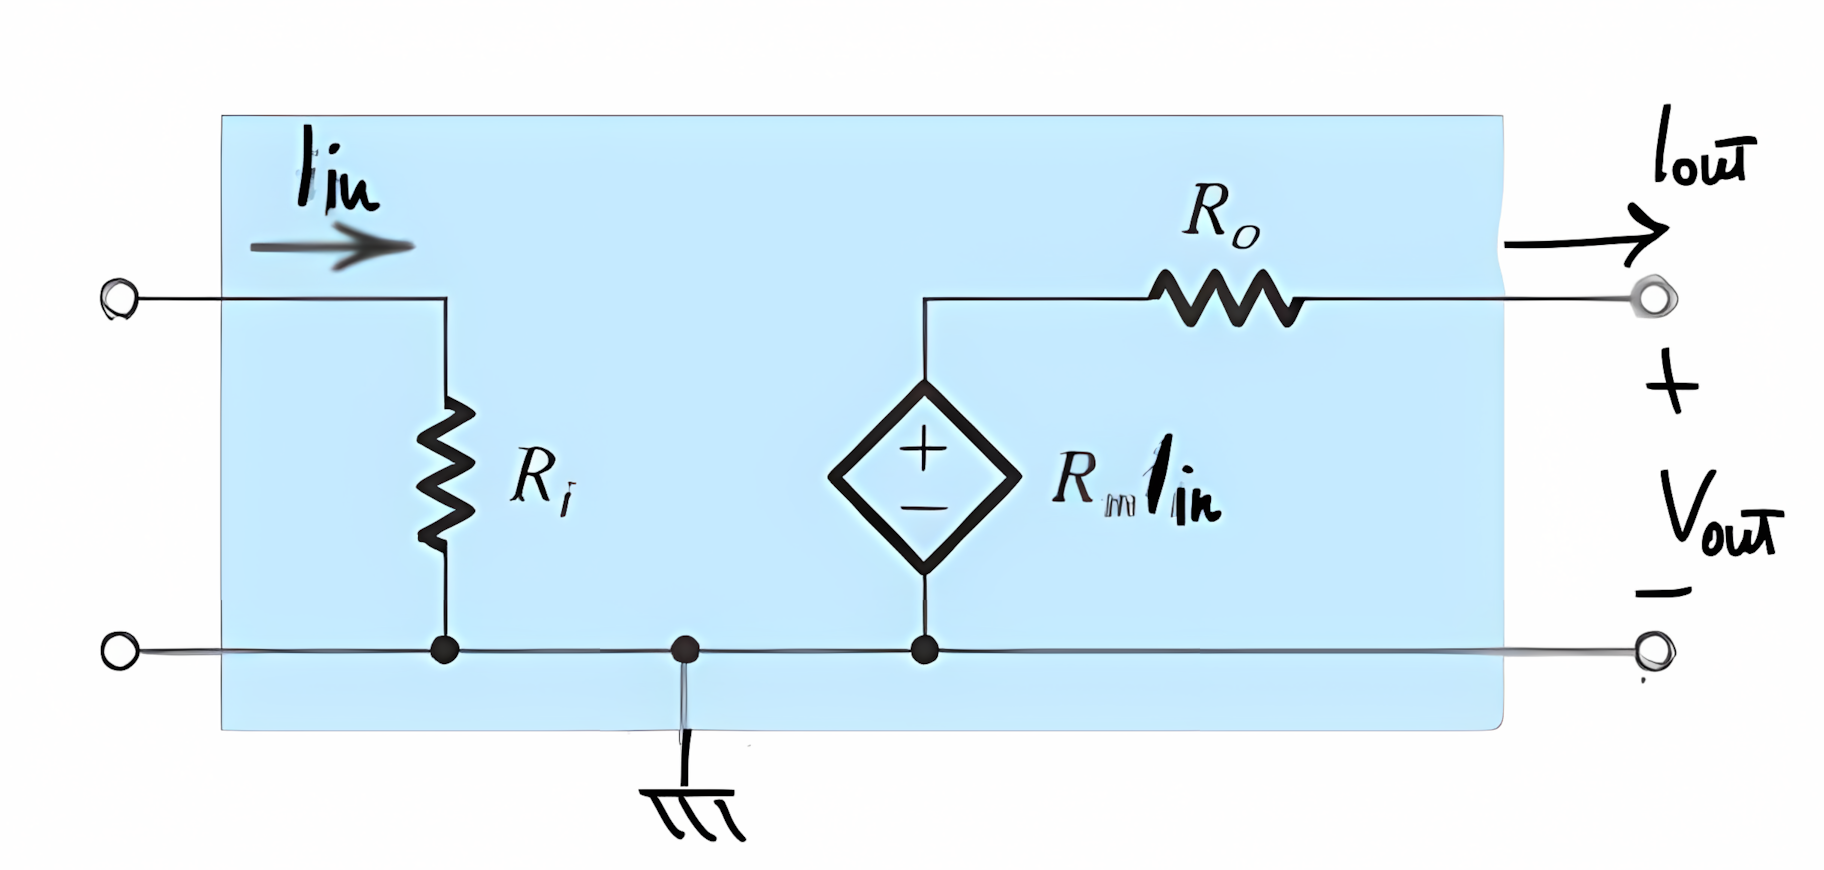
\includegraphics[width=0.6\textwidth]{images/1.2.1.1.png}
    \caption{Schema equivalente “rete due porte” di un amplificatore di transresistenza.}
    \label{fig:transresistenza}
\end{figure}

Idealmente, per non alterare il segnale in ingresso e non creare partitori di tensione, si desidera:
\[
R_i = 0, \quad R_o = 0.
\]
La configurazione invertente dell'amplificatore operazionale è la più idonea, in quanto offre una resistenza d’ingresso pari a \(R_1\) (vedi Figura~\ref{fig:transresistenza}a), mentre la configurazione non invertente presenta una resistenza d’ingresso infinita (Figura~\ref{fig:transresistenza}b). In entrambi i casi, la resistenza di uscita è nulla.
\newpage

\subsection{Amplificatore operazionale non invertente (Solo scritto)}

Si consideri il circuito illustrato in Figura~\ref{fig:non_inverting_amp}, dove il segnale in ingresso \(V_{\text{in}}\) è applicato direttamente al morsetto non invertente dell’operazionale, mentre il morsetto invertente è collegato all’uscita \(V_{\text{out}}\) tramite un resistore di retroazione e, contemporaneamente, connesso a massa attraverso un secondo resistore.\\[2mm]
\begin{figure}[H]
    \centering
    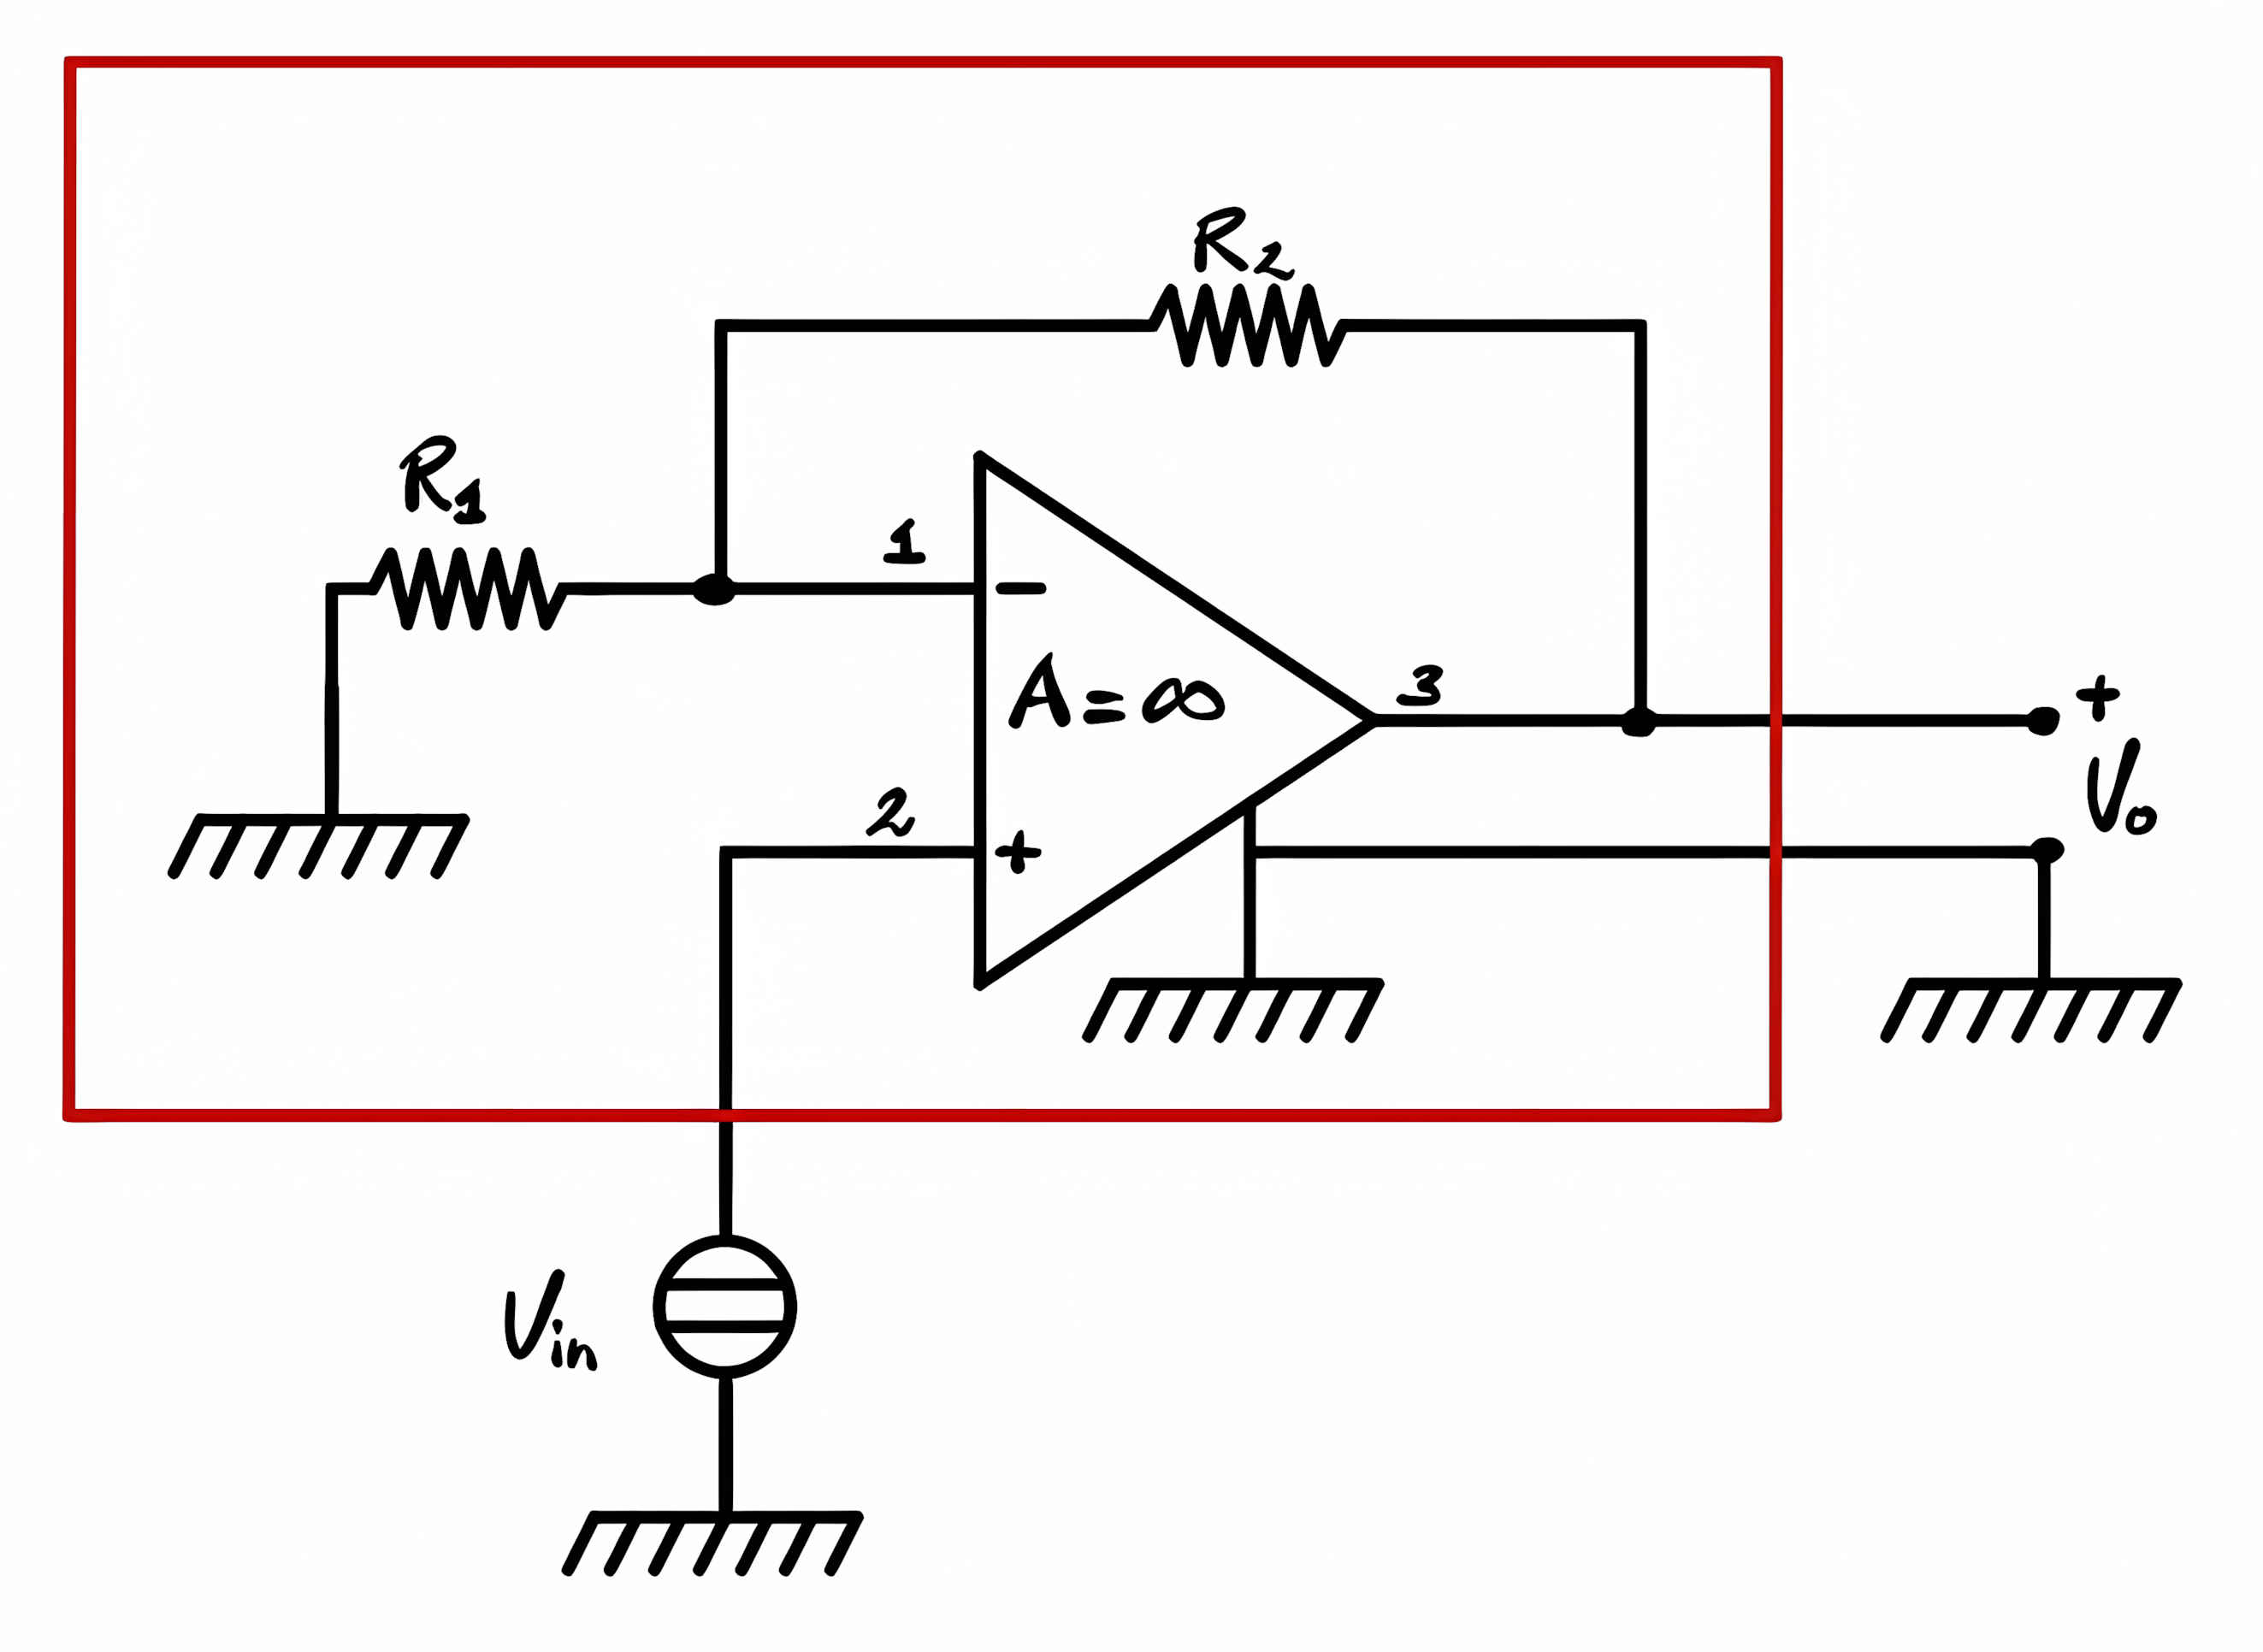
\includegraphics[width=0.6\textwidth]{images/1.2.2.1.png}
    \caption{Amplificatore operazionale in configurazione non invertente.}
    \label{fig:non_inverting_amp}
\end{figure}

In regime ideale, l’amplificatore operazionale si caratterizza per un guadagno a circuito aperto elevatissimo e per un’assenza di assorbimento di corrente ai morsetti di ingresso. 

Nella configurazione non invertente, il morsetto invertente tende ad assumere la stessa tensione del morsetto non invertente (principio di cortocircuito virtuale), per cui esso si trova sostanzialmente a \(V_{\text{in}}\). La corrente che circola nei resistori di retroazione risulta allora determinata unicamente dalle differenze di tensione fra l’uscita e l’ingresso, portando alla classica relazione che vincola \(V_{\text{out}}\) a \(V_{\text{in}}\). Sostituendo i valori di corrente nei due resistori e imponendo che la tensione ai morsetti di ingresso dell’operazionale sia la stessa, si giunge all’espressione:
\[
    V_{\text{out}} \;=\; V_{\text{in}} 
    \,\Bigl(1 + \tfrac{R_{2}}{R_{1}}\Bigr),
\]
dove \(R_{1}\) è il resistore tra morsetto invertente e massa, mentre \(R_{2}\) è quello fra l’uscita e il morsetto invertente.

Tale formula mostra chiaramente che la configurazione non invertente non introduce inversione di fase ed esibisce un guadagno in ampiezza pari a \(1 + \tfrac{R_{2}}{R_{1}}\). L’uscita risulta dunque proporzionale all’ingresso, con la costante di proporzionalità determinata dai due resistori in retroazione.
\newpage

\subsection{Parametri ideali di un amplificatore di tensione non invertente (Solo scritto)}

Quando l’amplificatore operazionale non invertente è considerato ideale, si assumono alcune proprietà che semplificano ulteriormente l’analisi del circuito. In particolare, l’impedenza di ingresso tende a essere molto elevata poiché, in prima approssimazione, nessuna corrente fluisce nel morsetto non invertente. Questa caratteristica fa sì che il carico posto in ingresso “veda” sostanzialmente un circuito aperto, evitando quasi ogni distorsione o attenuazione dovuta alla sorgente.

Parallelamente, l’impedenza di uscita si assume idealmente nulla, poiché l’operazionale, grazie alla retroazione, si comporta come un generatore di tensione pressoché perfetto: la tensione in uscita viene regolata in modo che i morsetti di ingresso rimangano a potenziali estremamente vicini tra loro. Di conseguenza, la disponibilità di corrente all’uscita è limitata solo dalle specifiche reali del componente, ma idealmente si assume che la tensione erogata non subisca cadute interne.

Il guadagno a circuito aperto molto elevato (\(A \rightarrow \infty\)) completa il quadro dell’idealità, poiché basta una piccolissima differenza di tensione tra morsetto invertente e non invertente per modificare drasticamente l’uscita. In virtù di tale caratteristica, la retroazione negativa costringe i due morsetti a mantenere la stessa tensione, generando esattamente il guadagno desiderato, che nella configurazione non invertente è
\[
    G \;=\; 1 + \frac{R_{2}}{R_{1}}.
\]

\newpage
%%%%%%%%%%%%%%%%%%%%%%%%%%%%%%%%%%%%%%%%%%%%%%%%%%%%%%%%%%%%%%%%%%%%%%%%%%%%%%%
\section{Filtri e Operazioni in Corrente}

\subsection{Struttura e funzionamento di un integratore}

Prendiamo il circuito di Figura~\ref{fig:integratore_ideale} composto da un amplificatore operazionale in configurazione invertente, dove è presente un condensatore \( C \) come impedenza di feedback.

Facendo l’ipotesi lineare, vale il cortocircuito virtuale, per cui i due morsetti dell’operazionale sono a 0 V. Ciò implica che ai capi di \( R_1 \) si stabilisce una caduta pari a \( V_{\text{in}} \), generando una corrente:
\[
I = \frac{V_{\text{in}}}{R_1}.
\]
Questa corrente va interamente nel condensatore \( C \), caricandolo. La tensione ai capi di \( C \) è data da:
\[
V_C = \frac{Q}{C} = \frac{1}{C} \int I(t) dt = \frac{1}{R_1 C} \int V_{\text{in}}(t) dt.
\]
Essendo definita \( V_{\text{out}} = -V_C \), la tensione di uscita risulta l’integrale della tensione d’ingresso, a meno di una costante moltiplicativa.

\begin{figure}[H]
    \centering
    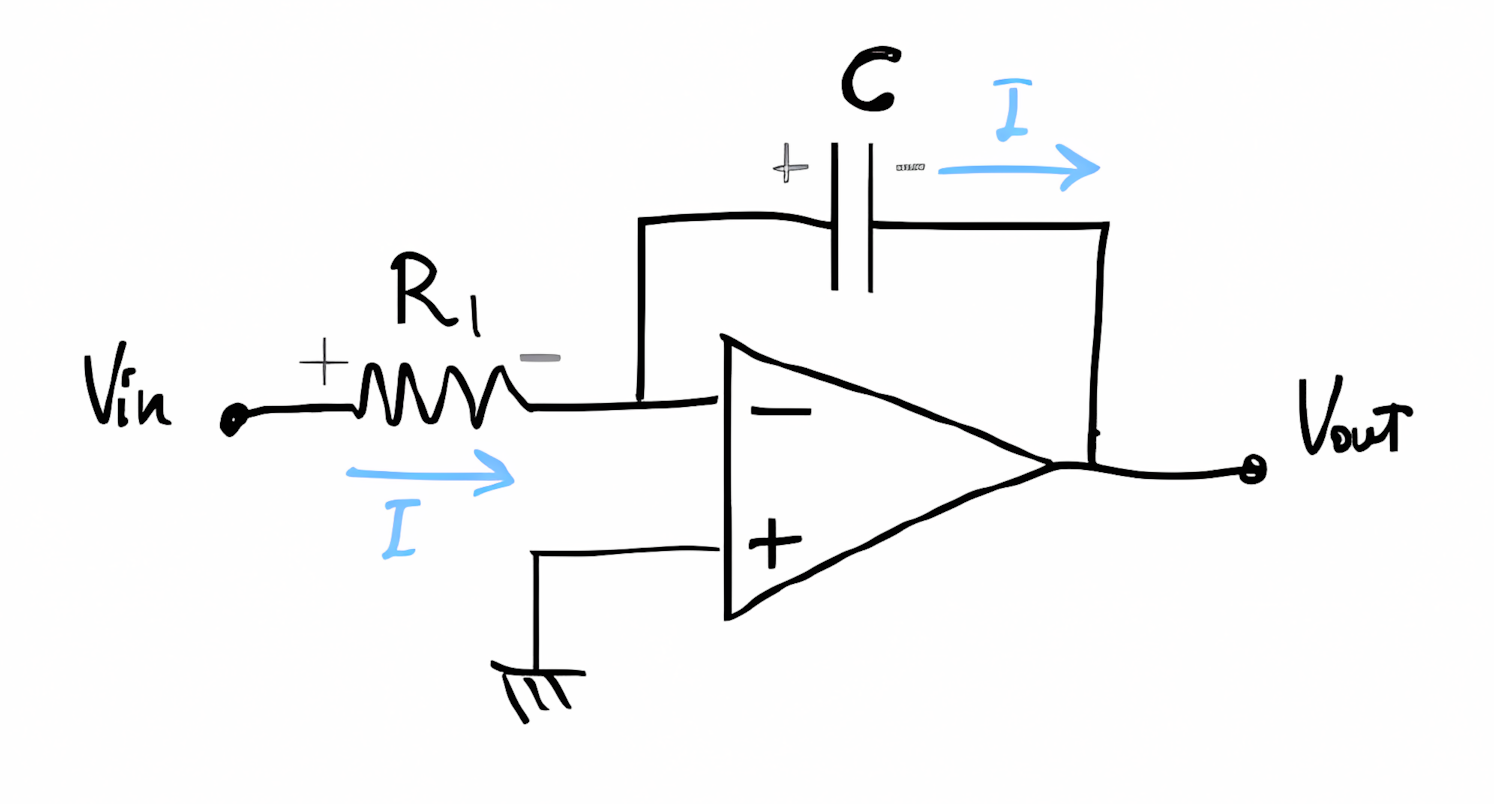
\includegraphics[width=0.5\linewidth]{images/1.3.1.1.png}
    \caption{Struttura di un integratore ideale.}
    \label{fig:integratore_ideale}
\end{figure}

Facendo un’analisi asintotica in funzione della frequenza del segnale in ingresso, vediamo che il guadagno è:
\[
A_v = \frac{Z_C}{R_1} = \frac{-1}{j \omega R_1 C}.
\]
Pertanto, per segnali a frequenza nulla (\( \omega = 0 \)) il guadagno è infinito, mentre per frequenze infinite il guadagno è nullo, ossia l’integratore si comporta come un passa basso.

Calcoliamo ora \( \omega_h \), definito come \( \omega_h = 1 / \tau = 1 / (R_{\text{eq}} C) \), dove \( R_{\text{eq}} \) è la resistenza equivalente vista dal condensatore. Se si sostituisce il condensatore con un generatore \( V_x \) (Fig. \ref{fig:integratore_g_ten}) e si annulla \( V_{\text{in}} \), si osserva che la corrente non scorre in \( R_1 \) (dato che entrambi i morsetti dell’A.O. sono a 0 V); di conseguenza, 
\[
R_{\text{eq}} = \infty \implies \omega_h = \frac{1}{\infty} = 0.
\]

\begin{figure}[H]
    \centering
    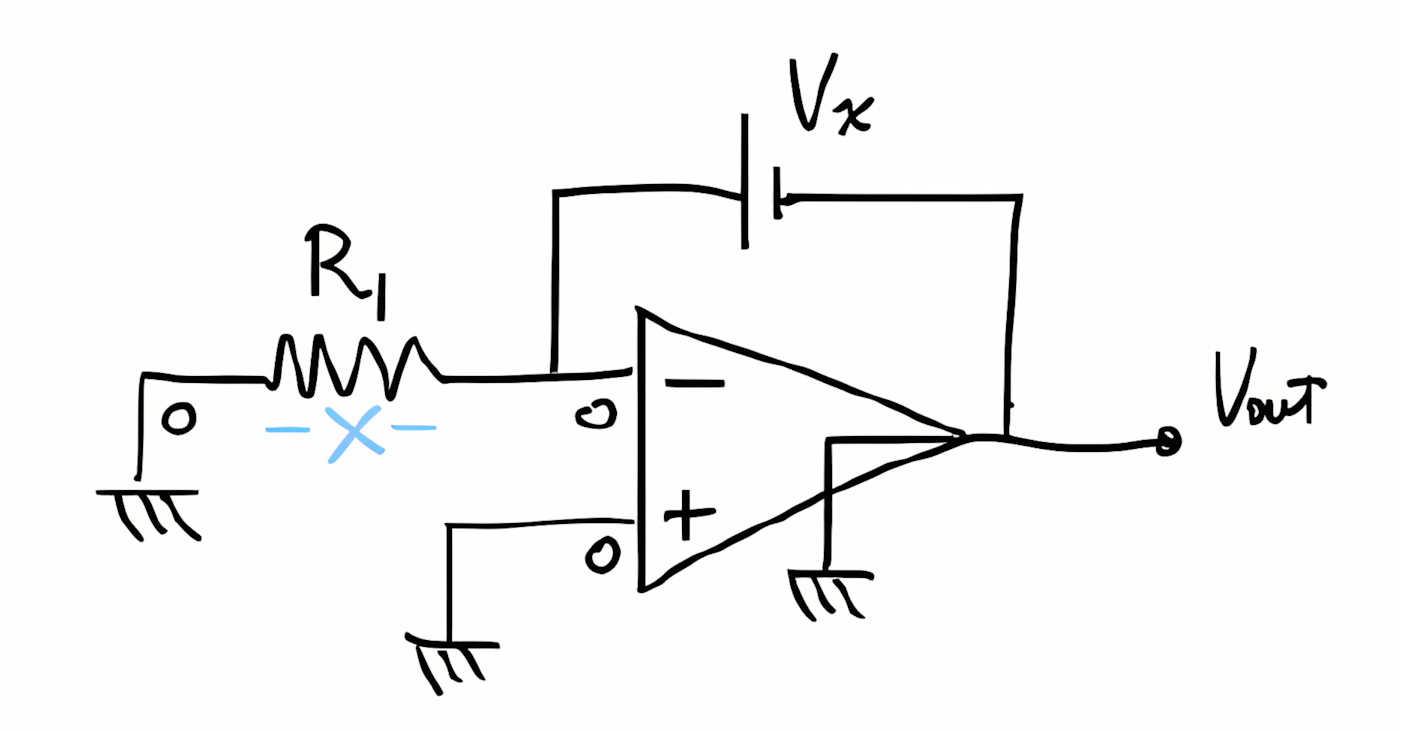
\includegraphics[width=0.5\linewidth]{images/1.3.1.2.png}
    \caption{Struttura di un integratore ideale (con approccio a generatore \(V_x\)).}
    \label{fig:integratore_g_ten}
\end{figure}

Questo significa che l’integratore ideale integra tutte le componenti, anche quelle di offset, portando a possibili saturazioni in presenza di rumore DC.

Per ovviare a questo problema, introduciamo l’integratore reale, che prevede una resistenza \( R_2 \) in parallelo al condensatore (vedi Figura~\ref{fig:integratore_reale}).\\[2mm]

In questo caso, la resistenza equivalente vista dal condensatore è \( R_2 \), perciò:
\[
\omega_h = \frac{1}{R_2 C},
\]
un valore finito (diverso da zero, come evidenziato in Figura~\ref{fig:integratore_reale}). In questo modo, tutte le componenti in frequenza inferiori a \( \omega_h \) sono semplicemente amplificate con guadagno \( A_v = -\frac{R_2}{R_1} \) e non integrate. Infatti, per \( \omega = 0 \), osserviamo che, una volta caricato il condensatore, tutta la corrente scorre su \( R_2 \), da cui:
\[
V_{\text{out}} = -V_{R_2} = -R_2 \frac{V_{\text{in}}}{R_1} \quad \implies \quad A_v = \frac{V_{\text{out}}}{V_{\text{in}}} = -\frac{R_2}{R_1}.
\]
\begin{figure}[H]
    \centering
    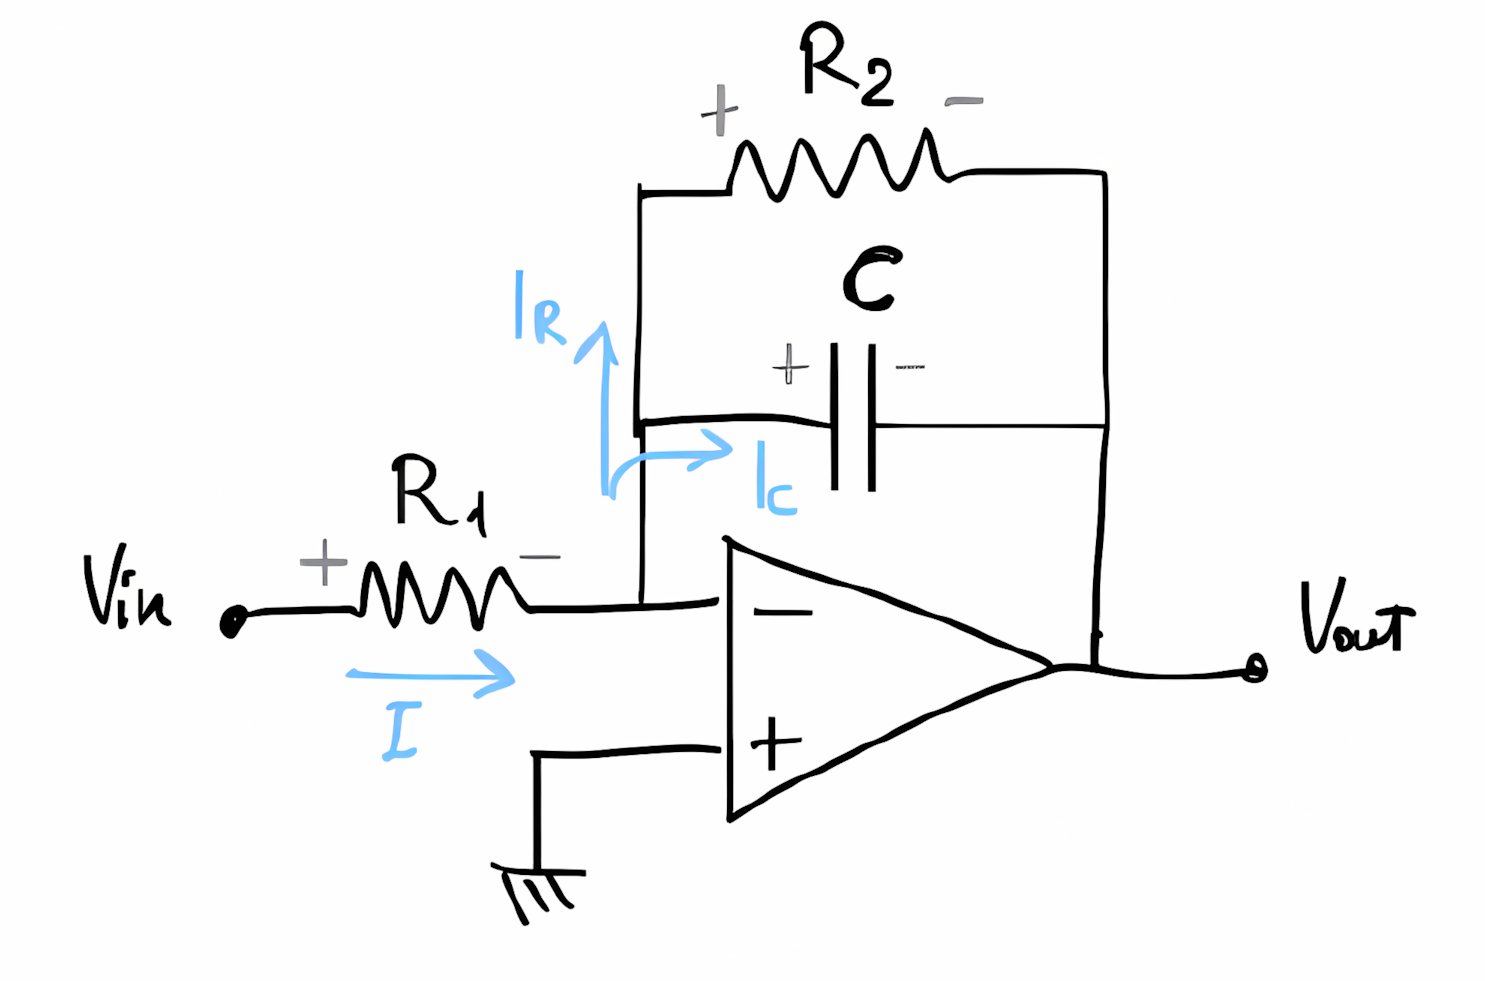
\includegraphics[width=0.5\linewidth]{images/1.3.1.3.png}
    \caption{Struttura di un integratore reale (con resistenza \( R_2 \) in parallelo).}
    \label{fig:integratore_reale}
\end{figure}
\newpage

\subsection{Funzionamento derivatore}

Il circuito derivatore, illustrato in Figura~\ref{fig:derivatore}, sfrutta un condensatore \( C \) come impedenza d’ingresso e una resistenza \( R_1 \) in retroazione. In questo modo, il condensatore realizza l’integrazione della corrente e, di conseguenza, la sua derivata viene trasferita all’uscita.\\[2mm]
\begin{figure}[H]
    \centering
    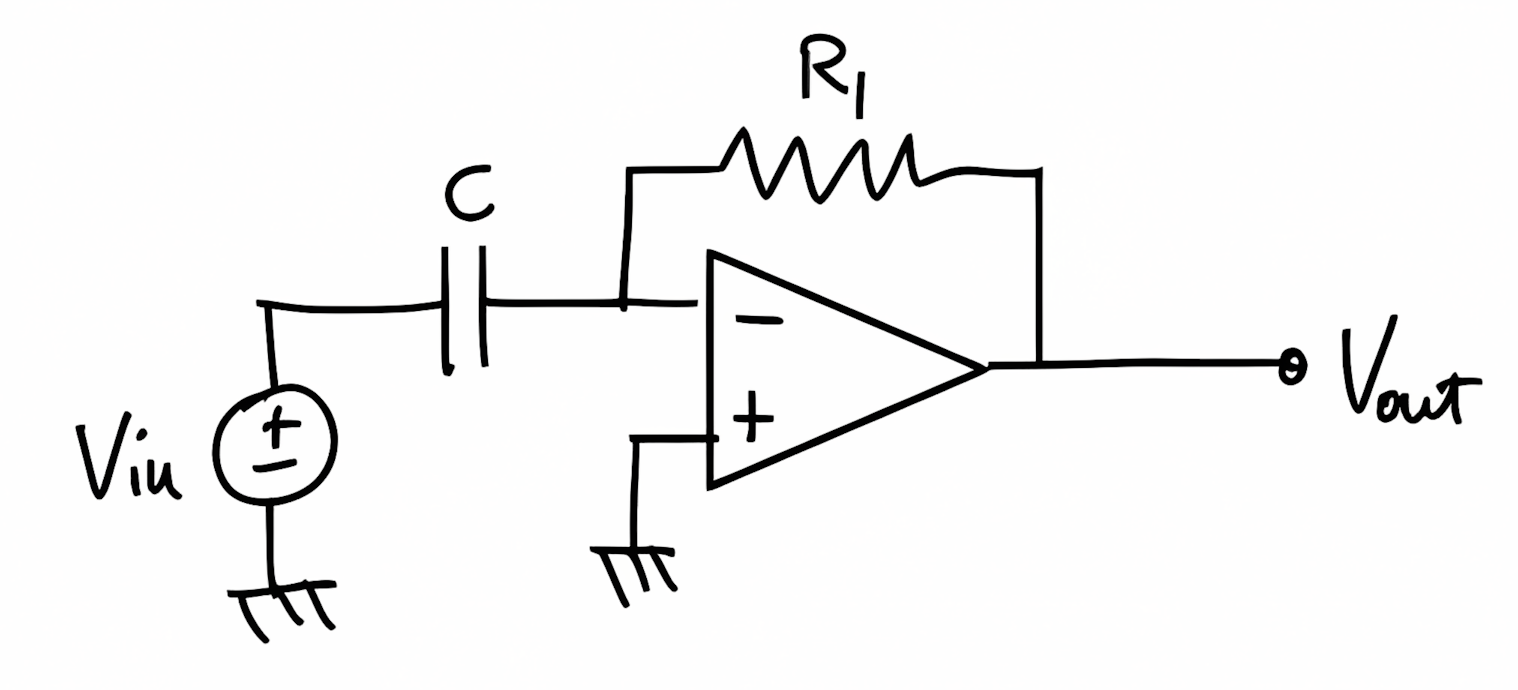
\includegraphics[width=0.6\textwidth]{images/1.3.2.1.png}
    \caption{Circuito derivatore.}
    \label{fig:derivatore}
\end{figure}

In particolare, la tensione ai capi del condensatore è data da
\[
V_C = \frac{Q}{C} = \frac{1}{C} \int I(t)\, dt,
\]
da cui, differenziando, si ottiene
\[
I(t) = C \frac{dV_C(t)}{dt}.
\]
Assumendo che, per il cortocircuito virtuale dell’operazionale, \( V_C \) coincida con il segnale d’ingresso \( V_{\text{in}} \), l'intera corrente \( I(t) \) scorre attraverso la resistenza \( R_1 \). Pertanto, la caduta su \( R_1 \) è
\[
V_{R_1} = R_1 I(t) = R_1 C \frac{dV_{\text{in}}(t)}{dt}.
\]
Essendo il circuito configurato in maniera invertente, l’uscita risulta:
\[
V_{\text{out}} = -V_{R_1} = -R_1 C \frac{dV_{\text{in}}(t)}{dt}.
\]
Così, l’uscita rappresenta, a meno di una costante, la derivata del segnale d’ingresso.

Il circuito si comporta come un passa-alto: il guadagno in frequenza è dato da
\[
A_v = \frac{V_{\text{out}}}{V_{\text{in}}} = \frac{R_1}{Z_C} = j \omega R_1 C,
\]
quindi per \(\omega=0\) il guadagno è nullo, mentre per \(\omega\to\infty\) tende all’infinito. Nel grafico della risposta in frequenza (Figura~\ref{fig:bode_derivatore}, parte a) il derivatore ideale mostra un guadagno che cresce linearmente con \(\omega\). In tale condizione, la frequenza di taglio si definisce come
\[
\omega_h = \frac{1}{\tau} = \frac{1}{R_{\text{eq}} C}.
\]
Nel derivatore ideale, tuttavia, la corrente non scorre in \( R_1 \) (per il cortocircuito virtuale), ottenendo \( R_{\text{eq}} = \infty \) e quindi \(\omega_h = 0\). Questo significa che tutte le componenti, incluse quelle indesiderate (come il rumore DC), vengono derivate, rischiando di saturare l’amplificatore.

Per ovviare a tale problema, è possibile limitare il guadagno alle alte frequenze introducendo una resistenza \( R_2 \) in serie (o in parallelo, a seconda della configurazione) al condensatore \( C \). In questo modo, la resistenza equivalente vista dal condensatore diventa \( R_2 \) e la frequenza di taglio risulta:
\[
\omega_h = \frac{1}{R_2 C},
\]
un valore finito (come illustrato in Figura~\ref{fig:derivatore_reale}). Con questa modifica, le componenti di frequenza inferiori a \(\omega_h\) vengono amplificate (o derivate) con un guadagno limitato, evitando problemi di saturazione.\\[2mm]
\begin{figure}[H]
    \centering
    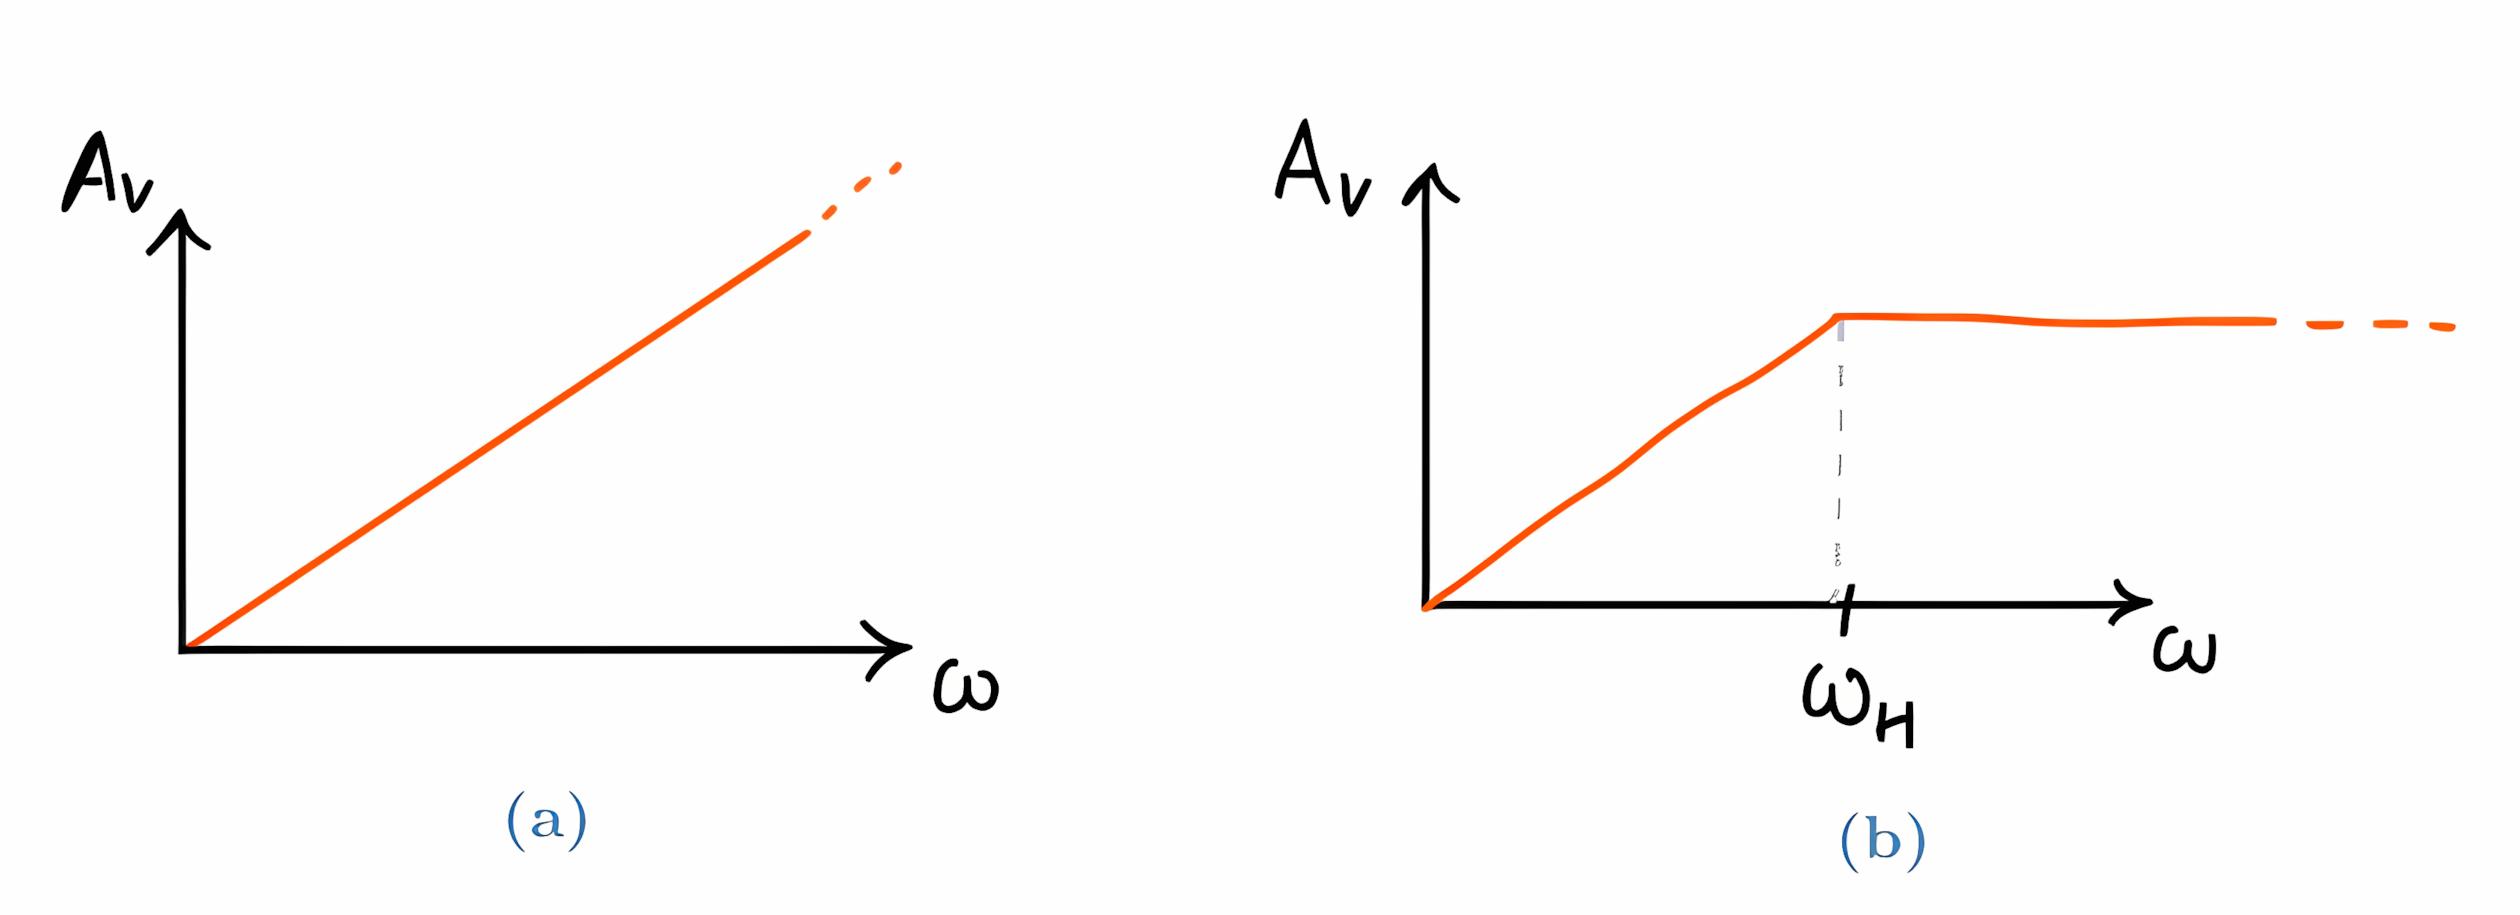
\includegraphics[width=0.6\textwidth]{images/1.3.2.2.png}
    \caption{Diagrammi di Bode in frequenza del derivatore ideale (a) e reale (b).}
    \label{fig:bode_derivatore}
\end{figure}

\begin{figure}[H]
    \centering
    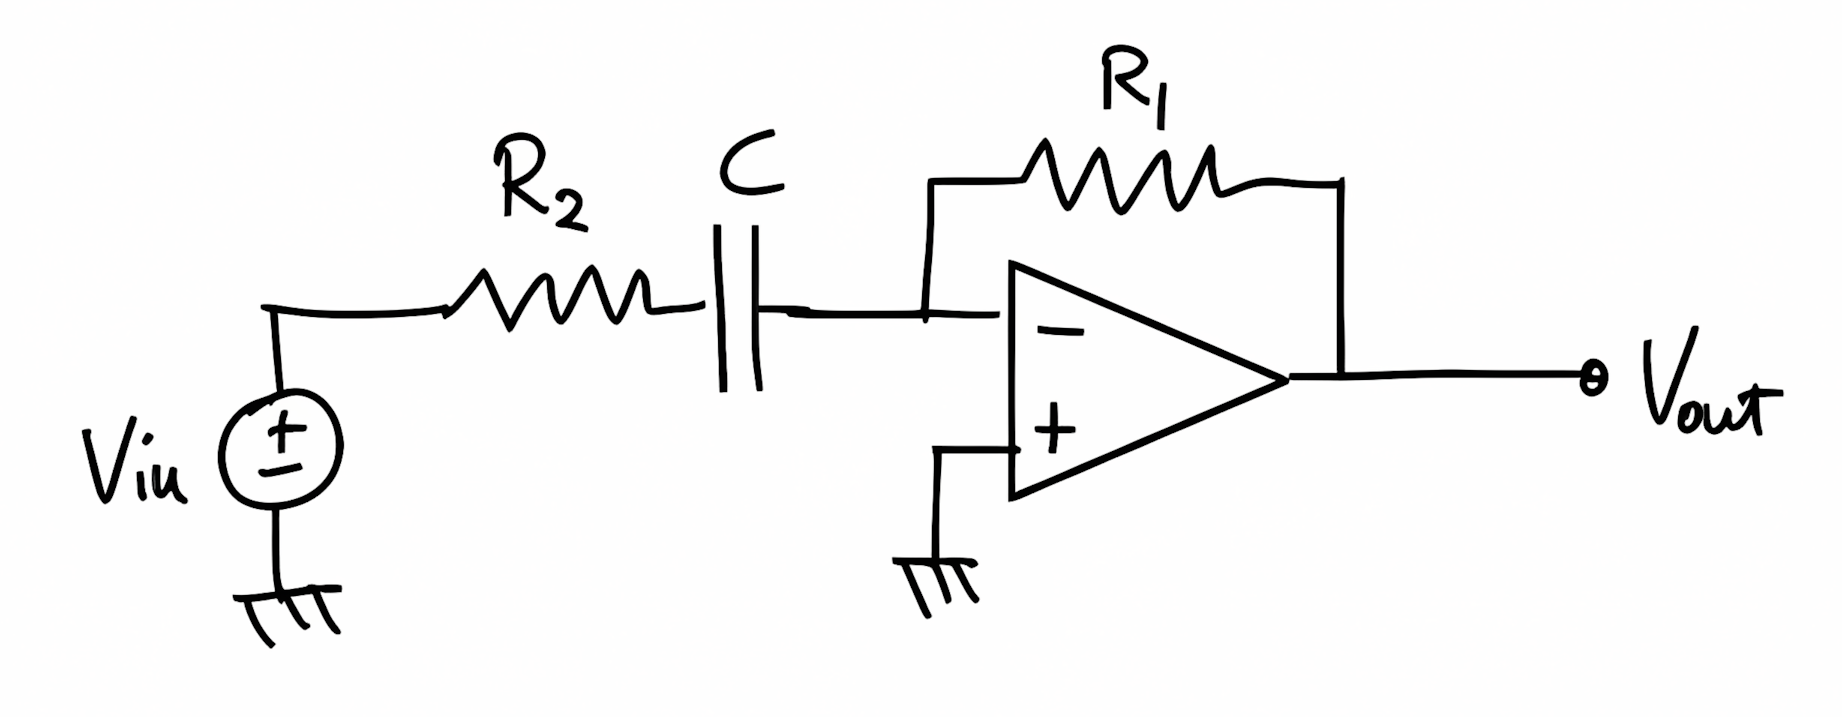
\includegraphics[width=0.6\textwidth]{images/1.3.2.3.png}
    \caption{Circuito derivatore reale.}
    \label{fig:derivatore_reale}
\end{figure}

\newpage

\subsection{Sommatore pesato invertente}

Un sommatore pesato (\ref{fig:sommatore}) invertente utilizza un amplificatore operazionale in configurazione invertente per ottenere in uscita una tensione che è la somma pesata di \( n \) tensioni in ingresso. In questo circuito il terminale non invertente è collegato a massa (0 V) e, grazie al principio del cortocircuito virtuale, il morsetto invertente si trova anch’esso a 0 V. Tale condizione permette di considerare, per ciascun ingresso, la caduta ai capi del resistore d’ingresso come uguale alla tensione fornita dal generatore.

\begin{figure}[H]
    \centering
    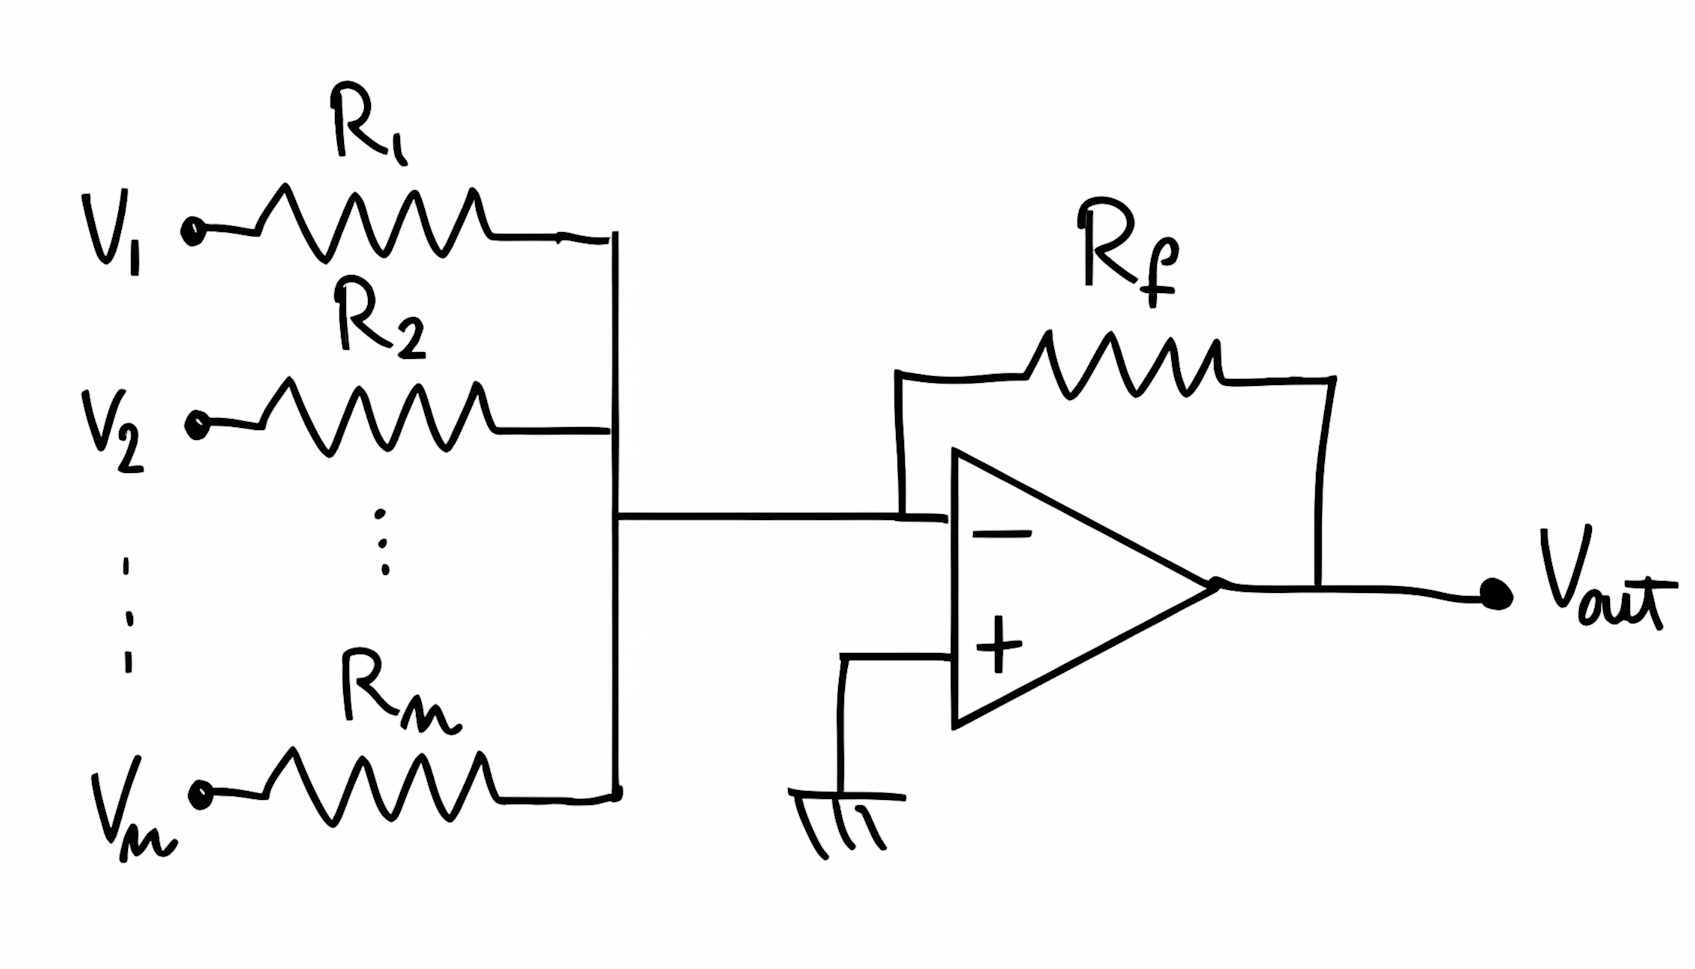
\includegraphics[width=0.6\textwidth]{images/1.3.3.1.png}
    \caption{Circuito sommatore pesato.}
    \label{fig:sommatore}
\end{figure}

Consideriamo il contributo di un generatore \( V_1 \) collegato tramite la resistenza \( R_1 \) al nodo invertente. Poiché il nodo si trova a 0 V, la differenza di potenziale ai capi di \( R_1 \) è semplicemente \( V_1 \) (cioè \( V_1 - 0 = V_1 \)). Di conseguenza, la corrente \( I_1 \) che scorre da \( V_1 \) al nodo invertente è data da
\[
I_1 = \frac{V_1}{R_1}.
\]
Dato che l’amplificatore operazionale ha un’impedenza d’ingresso molto elevata e non assorbe corrente, la corrente \( I_1 \) non ha altre vie per fluire se non attraverso la resistenza di retroazione \( R_f \). Quindi, la stessa corrente \( I_1 \) attraversa \( R_f \), generando una caduta di tensione
\[
V_{R_f} = I_1 \, R_f = \frac{R_f}{R_1}\, V_1.
\]
Essendo il circuito configurato in maniera invertente, la tensione d’uscita dovuta al generatore \( V_1 \) risulta:
\[
V_0(V_1 \neq 0) = - V_{R_f} = -\frac{R_f}{R_1}\, V_1.
\]

Lo stesso ragionamento vale per ogni generatore di tensione collegato all’ingresso. Se, ad esempio, consideriamo un generatore \( V_2 \) con la relativa resistenza \( R_2 \), si ottiene:
\[
V_0(V_2 \neq 0) = -\frac{R_f}{R_2}\, V_2,
\]
e in generale per l'\( i \)-esimo ingresso:
\[
V_0(V_i \neq 0) = -\frac{R_f}{R_i}\, V_i.
\]

Poiché il circuito è lineare, il principio di sovrapposizione degli effetti vale: si possono considerare i contributi di ciascun generatore separatamente, cortocircuitando gli altri (ovvero, sostituendoli con un collegamento a massa). Sommando linearmente i contributi si ottiene l’espressione complessiva per l’uscita:
\[
V_0 = -\frac{R_f}{R_1}\, V_1 - \frac{R_f}{R_2}\, V_2 - \cdots - \frac{R_f}{R_n}\, V_n = -\sum_{i=1}^{n} \frac{R_f}{R_i}\, V_i.
\]
\newpage
%%%%%%%%%%%%%%%%%%%%%%%%%%%%%%%%%%%%%%%%%%%%%%%%%%%%%%%%%%%%%%%%%%%%%%%%%%%%%%%
\section{Specchi e Altri Circuiti Analogici}

\subsection{Specchio di corrente}

Lo specchio di corrente permette di ottenere una corrente \(I\) a partire da una corrente di riferimento \(I_{\text{ref}}\). Si realizza, ad esempio, utilizzando due NMOS \(Q_1\) e \(Q_2\) con il gate comune, dove il drain di \(Q_1\) è collegato al gate. In questo modo \(Q_1\) opera in saturazione (vedi nota a piè di pagina).

Assumendo \(V_{G1} = V_{G2}\) (cioè \(V_{GS1} = V_{GS2}\)), se \(Q_2\) è in saturazione si ha:
\[
I = k_2 (V_{GS} - V_t)^2,
\]
mentre per \(Q_1\) (in saturazione) è
\[
I_{\text{ref}} = k_1 (V_{GS} - V_t)^2.
\]
Pertanto:
\[
I = \frac{k_2}{k_1} I_{\text{ref}}.
\]
Questo approccio è vantaggioso quando occorre generare diverse correnti \(I_1,\dots,I_n\) a partire da un'unica sorgente \(I_{\text{ref}}\).\\[2mm]
\begin{figure}[H]
    \centering
    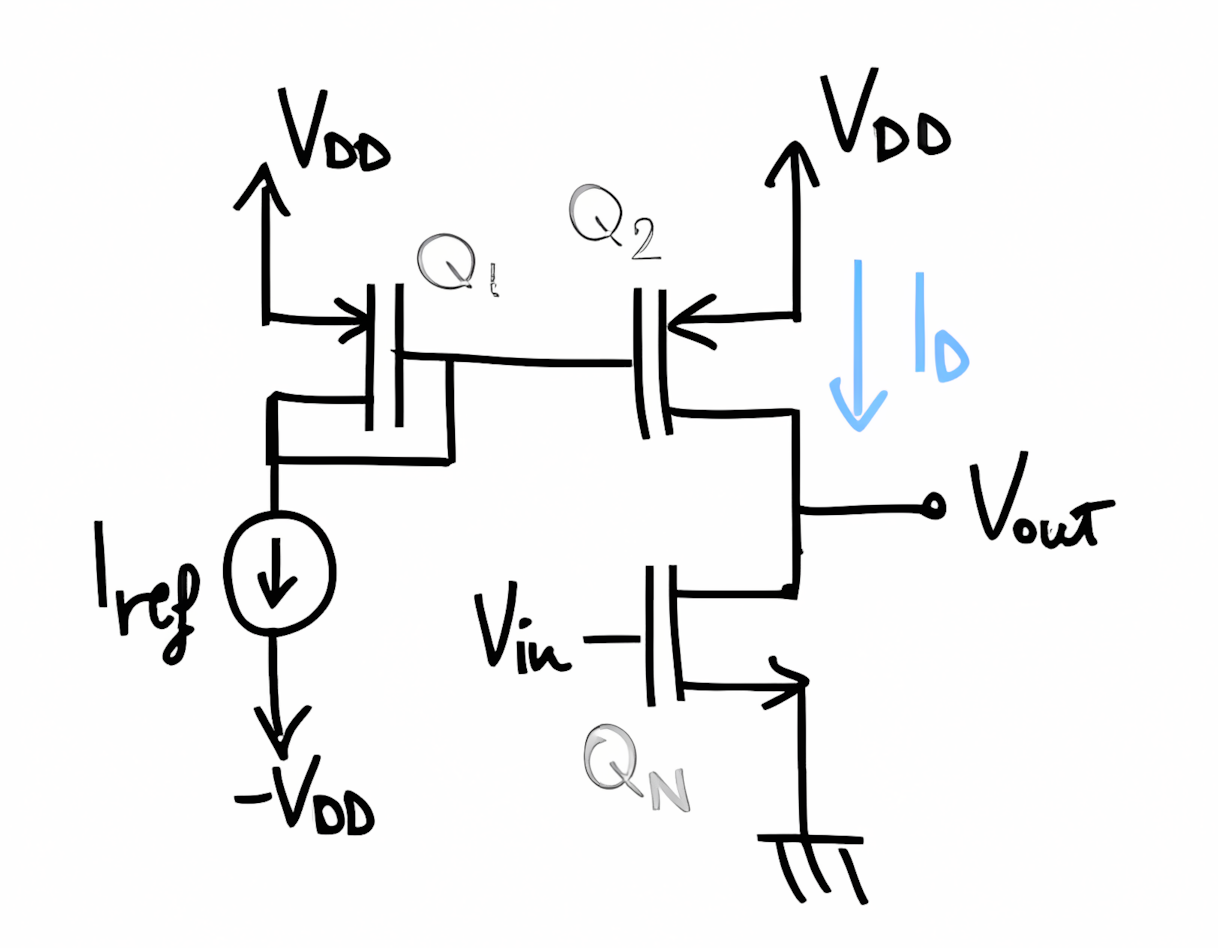
\includegraphics[width=0.6\textwidth]{images/1.4.1.1.png}
    \caption{Struttura dello specchio di corrente con due NMOS.}
    \label{fig:specchio_corrente}
\end{figure}

\begin{figure}[H]
    \centering
    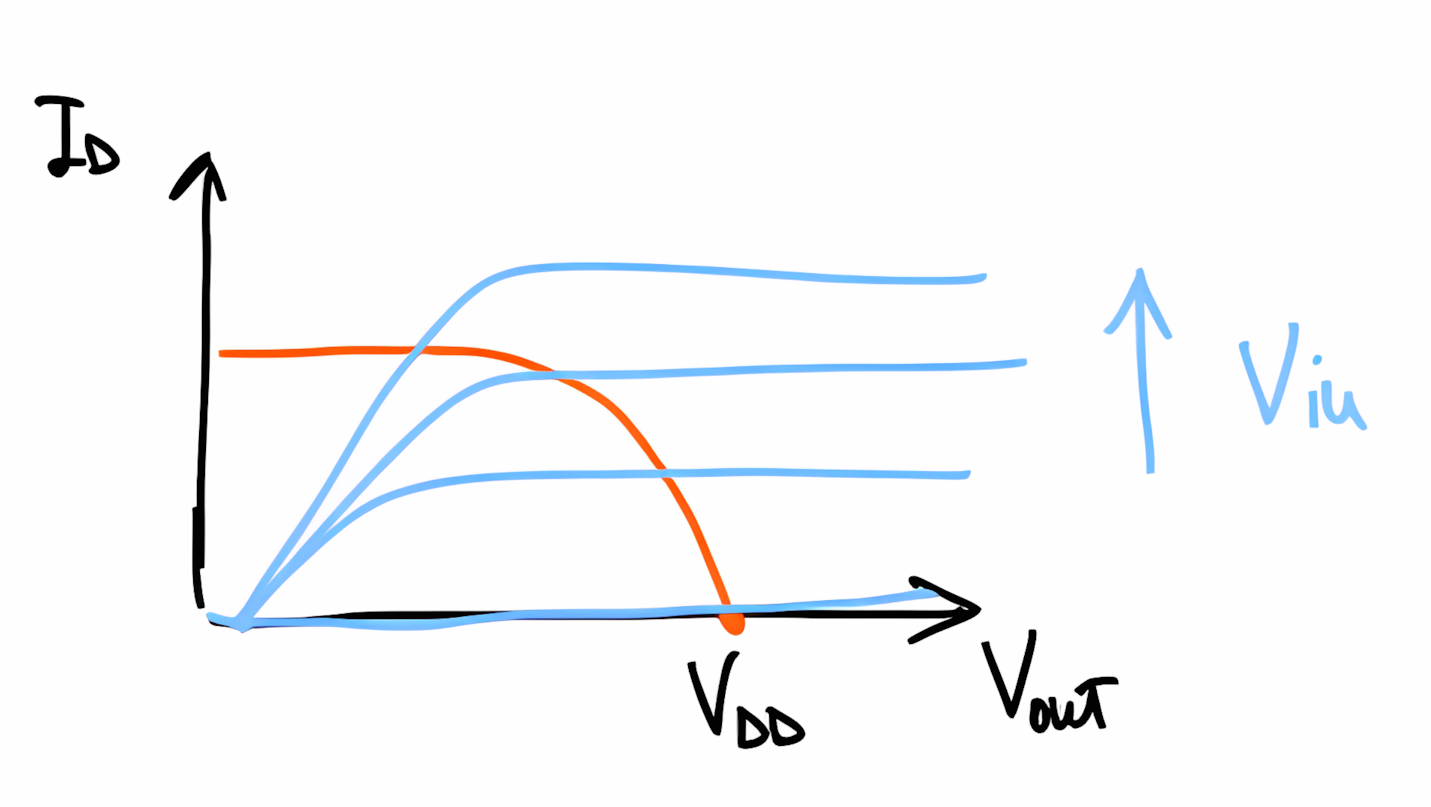
\includegraphics[width=0.6\textwidth]{images/1.4.1.2.png}
    \caption{Transcaratteristica dello specchio di corrente.}
    \label{fig:specchio_corrente_tc}
\end{figure}

\newpage

\subsection{Transistor MOS a svuotamento}
Un transistor MOS a svuotamento ha una struttura simile a quella di un transistor MOS ad arricchimento, con la differenza che il canale che collega le isole di drain e source è presente anche in assenza di una tensione applicata al gate. In altre parole, il canale viene creato al momento della costruzione del dispositivo, formando una zona di tipo \(n\) (oppure di tipo \(p\), a seconda del modello) tra le due isole; per questo motivo si dice che il transistor è \emph{normalmente on}, poiché la corrente scorre sempre anche se non viene applicata alcuna tensione al gate.
\begin{figure}[H]
  \centering
  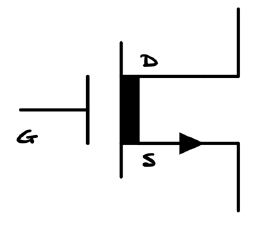
\includegraphics[width=0.5\textwidth]{images/1.4.2.2.png}
  \caption{Simbolo circuitale di un transistor MOS a svuotamento.}
  \label{fig:mos_depletion_symbol}
\end{figure}
Applicando una tensione sul gate si modificano le condizioni di scorrimento della corrente. Nel caso di un transistor NMOS, una tensione positiva sul gate aumenta il numero di cariche elettriche nel canale di tipo \(n\), riducendo la resistenza e aumentando la corrente di drain. Al contrario, applicando una tensione negativa il campo elettrico allontana le cariche di tipo \(n\), aumentando la resistenza e diminuendo la corrente di drain. Quando la tensione \(V_{GS}\) scende al di sotto di una certa soglia, si verifica un’inversione di tipo: il canale preesistente di tipo \(n\) diventa di tipo \(p\) a causa del campo elettrico che respinge le cariche negative e attira le lacune del substrato. Di conseguenza, la caratteristica \(I_D\) in funzione di \(V_{DS}\) non è nulla per \(V_{GS}=0\), ma diventa nulla se \(V_{GS}\) scende al di sotto della soglia; analogamente, la caratteristica \(I_D\) in funzione di \(V_{GS}\) assume la forma di una parabola (con un solo ramo) il cui vertice è spostato verso tensioni negative.

Il simbolo circuitale di un transistor MOS a svuotamento è mostrato in Figura~\ref{fig:mos_depletion_symbol} e evidenzia che il canale tra drain e source è preesistente.

\begin{figure}[H]
  \centering
  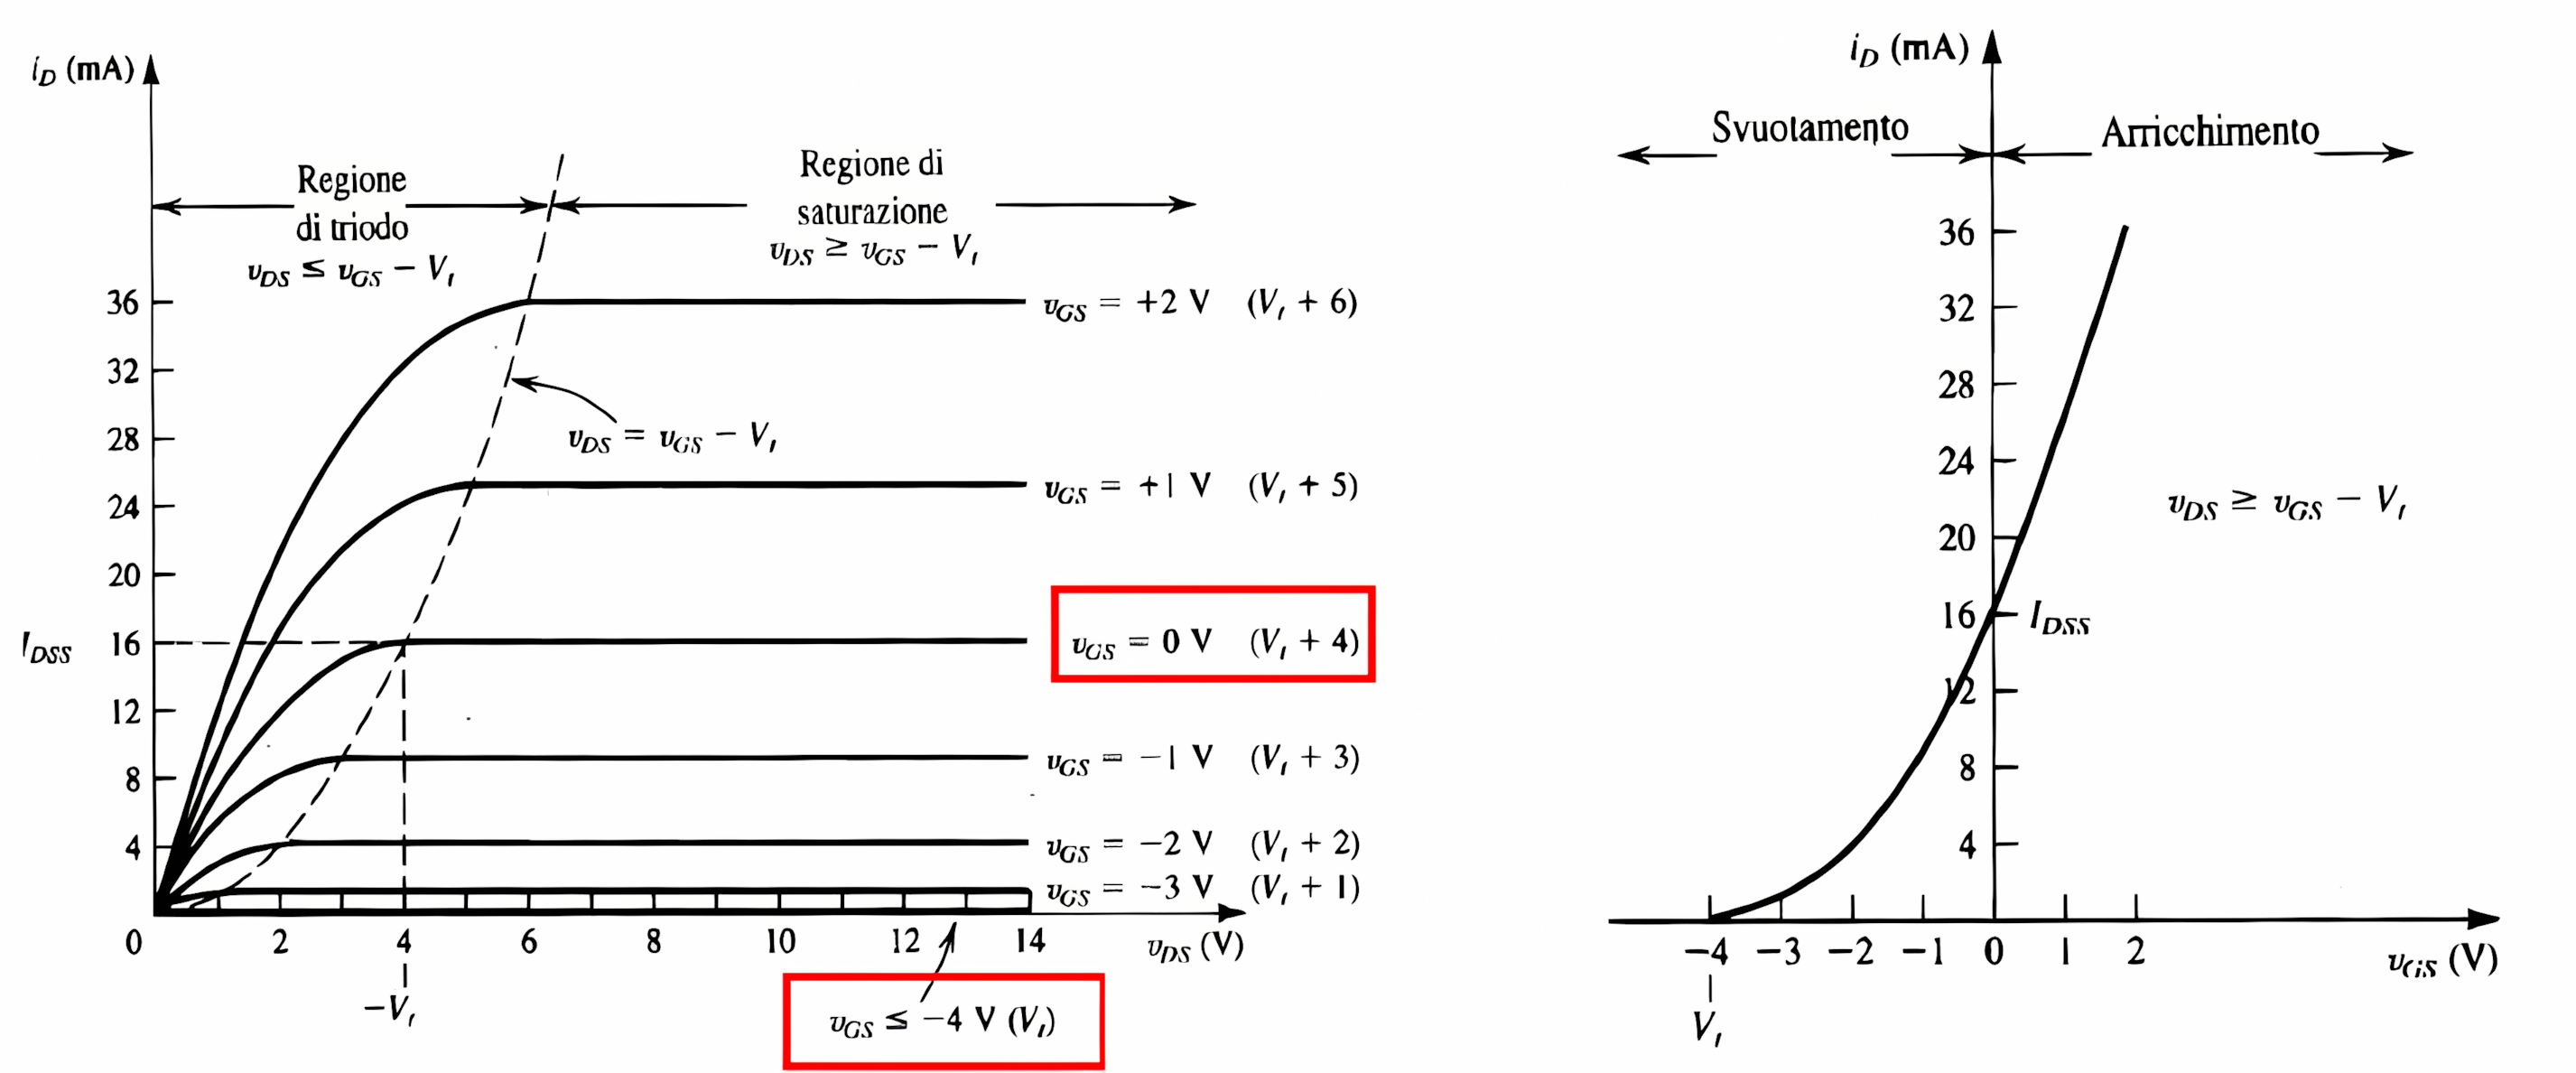
\includegraphics[width=1\textwidth]{images/1.4.2.1.png}
  \caption{Transcaratteristica di un transistor MOS a svuotamento.}
  \label{fig:transc_svuot}
\end{figure}
\newpage
%%%%%%%%%%%%%%%%%%%%%%%%%%%%%%%%%%%%%%%%%%%%%%%%%%%%%%%%%%%%%%%%%%%%%%%%%%%%%%%
\section{Amplificatori Differenziali e per Strumentazione}

\subsection{Funzionamento di un amplificatore differenziale}

Un amplificatore differenziale amplifica la differenza tra due segnali \(V_1\) e \(V_2\). In generale l'output può essere scritto come:
\[
V_{\text{out}} = A_{\text{CM}} \left(\frac{V_1+V_2}{2}\right) + A_D (V_2-V_1),
\]
mentre in un amplificatore idealmente differenziale \(A_{\text{CM}} = 0\). La realizzazione del circuito è mostrata in Figura~\ref{fig:amp_diff}.\\[2mm]
\begin{figure}[H]
    \centering
    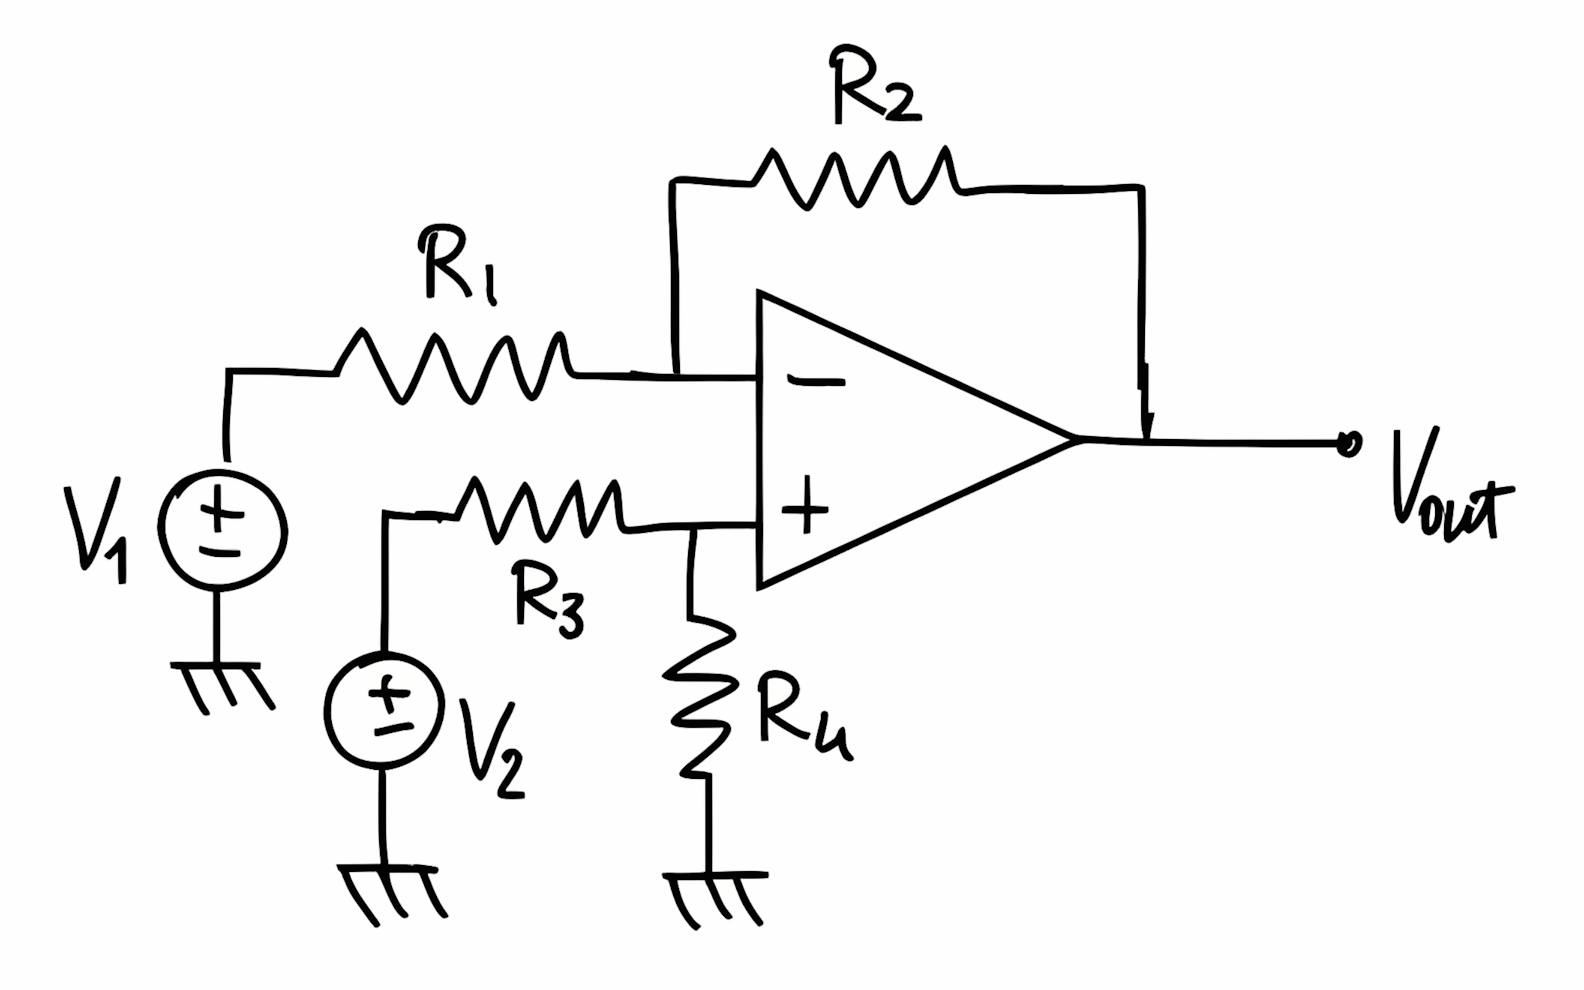
\includegraphics[width=0.6\textwidth]{images/1.5.1.1.png}
    \caption{Circuito per la realizzazione di un amplificatore differenziale idealmente.}
    \label{fig:amp_diff}
\end{figure}

Applicando il principio di sovrapposizione, si ottiene:
\[
V_{\text{out}} = -\frac{R_2}{R_1} V_1 + \left(1+\frac{R_2}{R_1}\right)\frac{R_4}{R_3+R_4}V_2.
\]
L'idealità (cioè \(V_1=V_2 \implies V_{\text{out}}=0\)) richiede che il rapporto \(R_3/R_4\) sia uguale a \(R_1/R_2\), e il guadagno risulta:
\[
A_v = \frac{R_2}{R_1}(V_2-V_1).
\]
Per evitare problemi di impedenza agli ingressi, si possono disaccoppiare i generatori mediante buffer di tensione.
\newpage

\subsection{Amplificatore differenziale per strumentazione}

Un amplificatore differenziale è impiegato per effettuare misurazioni precise in presenza di un forte segnale di modo comune, ad esempio quando si desidera misurare la differenza di luminosità tra il punto in cui è accesa una candela e un punto sullo sfondo. Poiché l’amplificatore differenziale annulla il segnale di modo comune (cioè, \(A_{CM} \approx 0\)), si ottiene una misura accurata della differenza dei due segnali.\\[2mm]
\begin{figure}[H]
  \centering
  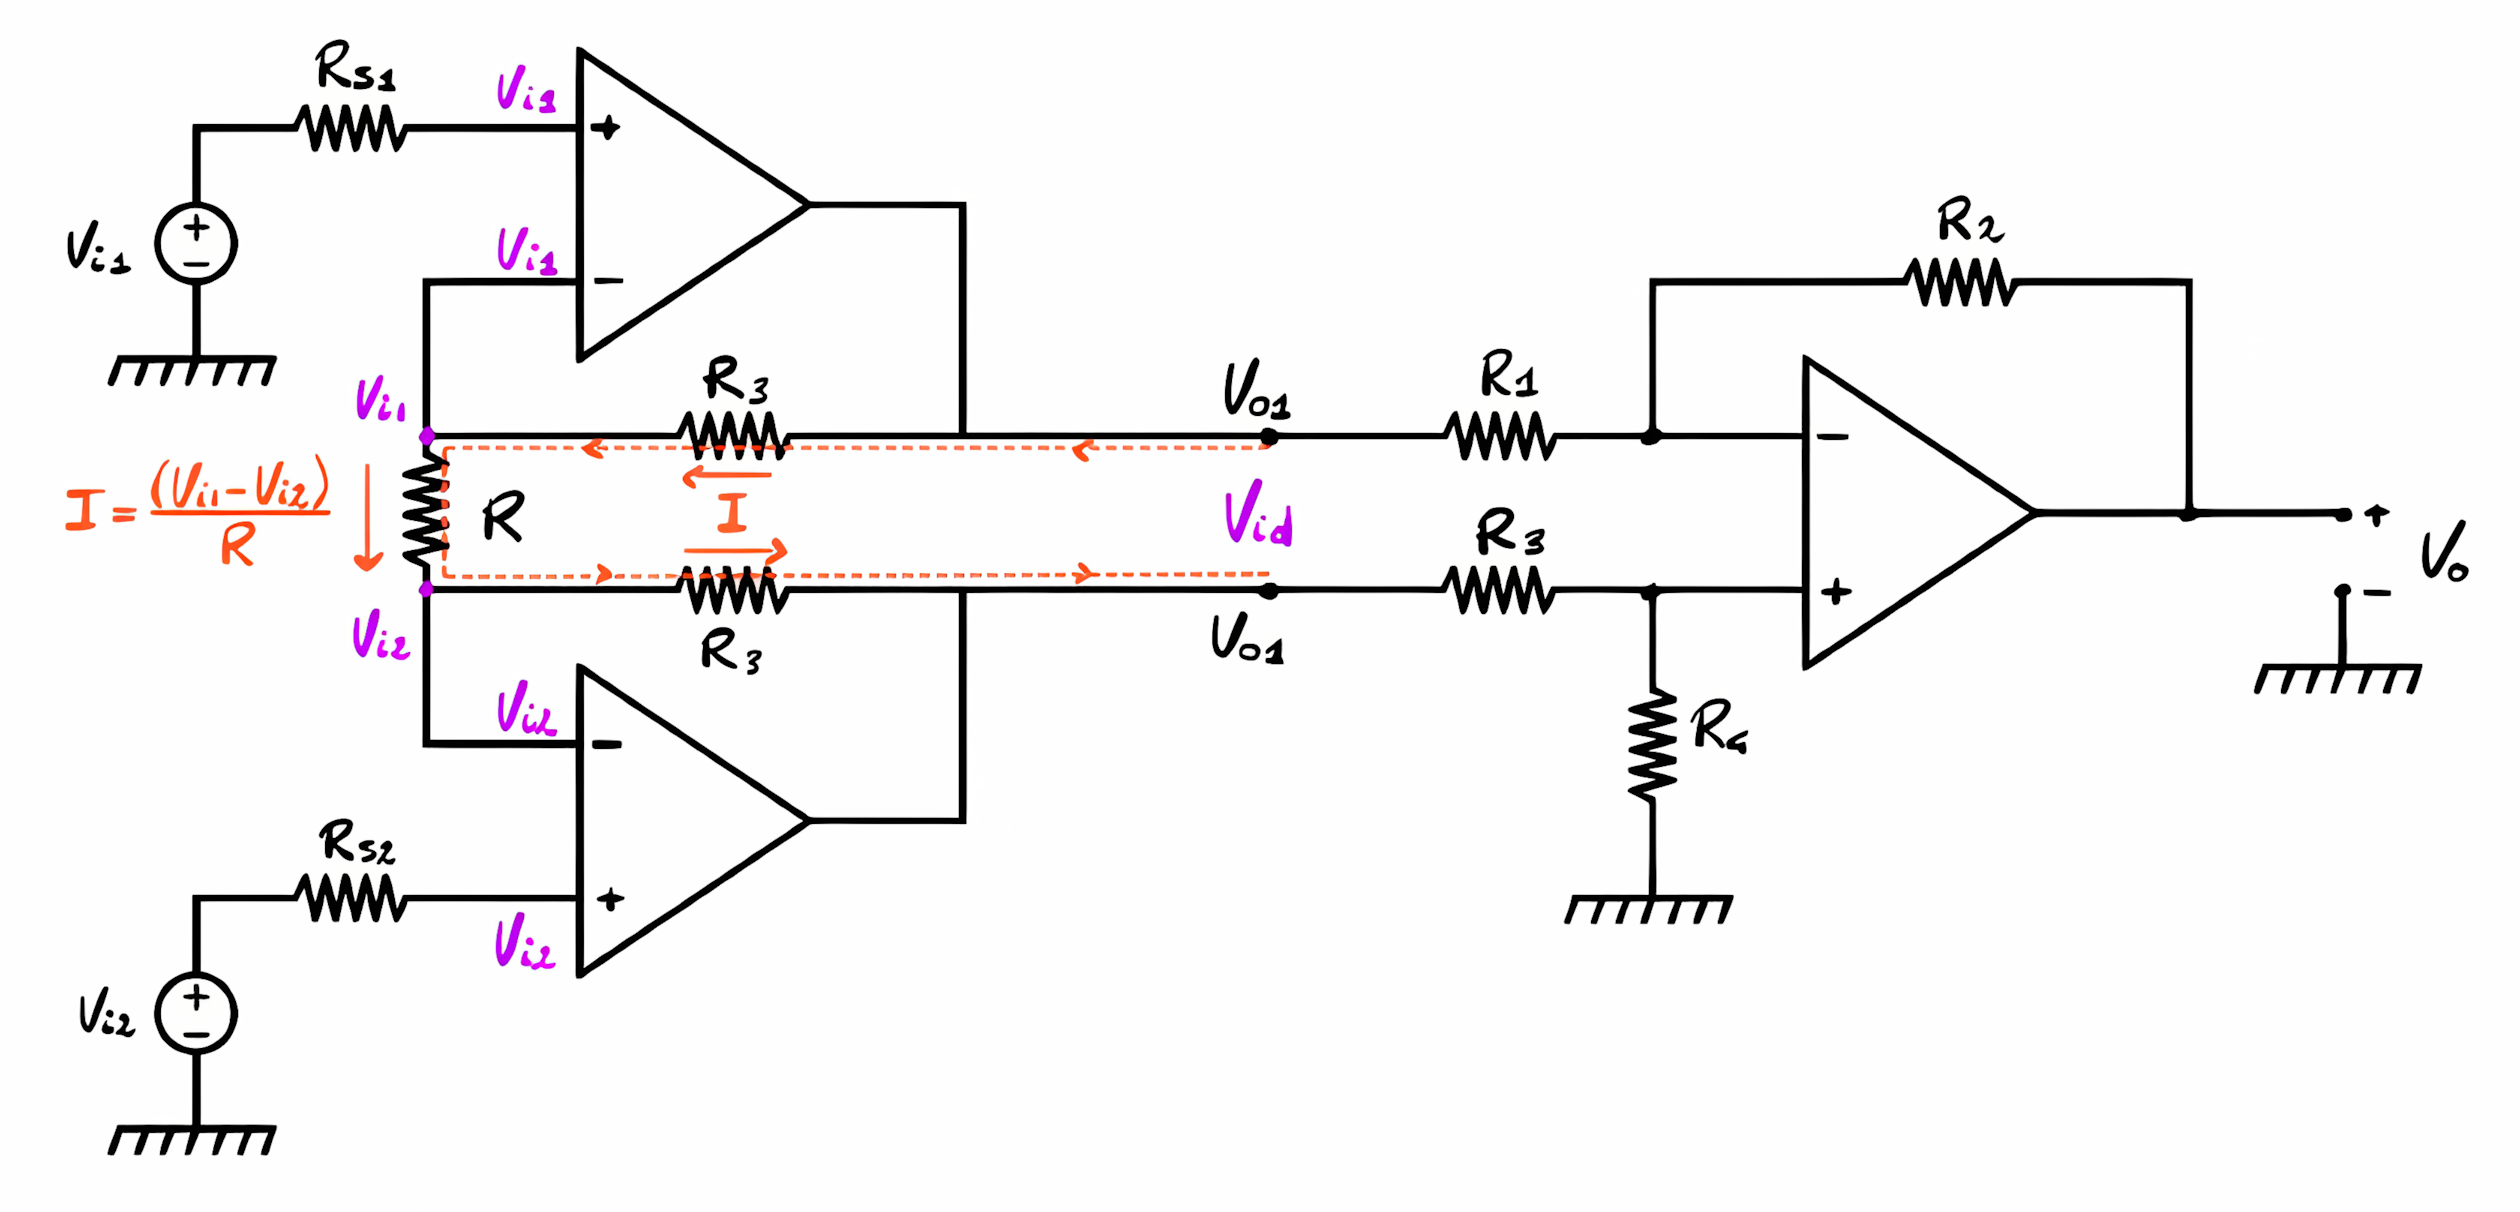
\includegraphics[width=0.7\textwidth]{images/1.5.2.1.png}
  \caption{Schema del circuito per strumentazione: \(R_1 = R_3\), \(R_2 = R_4\) sono costanti, mentre la resistenza \(R\) regola il guadagno.}
  \label{fig:amp_diff_strumentazione}
\end{figure}

Per il principio del cortocircuito virtuale, il potenziale nei morsetti dei buffer assume i valori \(V_{1+}\) e \(V_{2+}\) rispettivamente. La differenza \(V_{1+} - V_{2+}\) genera una corrente \(I\) che scorre attraverso la resistenza \(R\):
\[
I = \frac{V_{1+} - V_{2+}}{R}.
\]
Poiché tale corrente non può entrare o uscire dai morsetti degli amplificatori operazionali, essa deve necessariamente percorrere anche le resistenze \(R_3\) presenti nei rami di retroazione. Di conseguenza, la caduta complessiva sui rami è:
\[
V_{ad} = I R_3 + I R = I (R + 2R_3),
\]
ovvero, sostituendo \(I\),
\[
V_{ad} = (V_{1+} - V_{2+}) \cdot \frac{R + 2R_3}{R}.
\]

Infine, l’uscita dell’amplificatore differenziale, che opera in configurazione invertente, risulta:
\[
V_o = -\frac{R_2}{R_1} \left( 1 + \frac{2R_3}{R} \right) (V_{1+} - V_{2+}).
\]
In questo modo, il guadagno del circuito dipende unicamente dal valore della resistenza \(R\), che può essere regolata per ottenere il guadagno desiderato, mentre le coppie \(R_1 = R_3\) e \(R_2 = R_4\) rimangono fisse per preservare l’idealità del dispositivo.

\newpage
%%%%%%%%%%%%%%%%%%%%%%%%%%%%%%%%%%%%%%%%%%%%%%%%%%%%%%%%%%%%%%%%%%%%%%%%%%%%%%%
\section{Multivibratori e Forme d’Onda}

\subsection{Struttura e funzionamento di un multivibratore astabile con A.O. per forme d’onda triangolari}

Consideriamo un multivibratore astabile realizzato con un amplificatore operazionale in configurazione a controreazione positiva, il cui output iniziale è \(L^+\). Questo segnale alimenta un integratore (basato su A.O. con controreazione negativa tramite condensatore, vedi Figura~\ref{fig:onda_triangolare}).\\[2mm]
\begin{figure}[H]
    \centering
    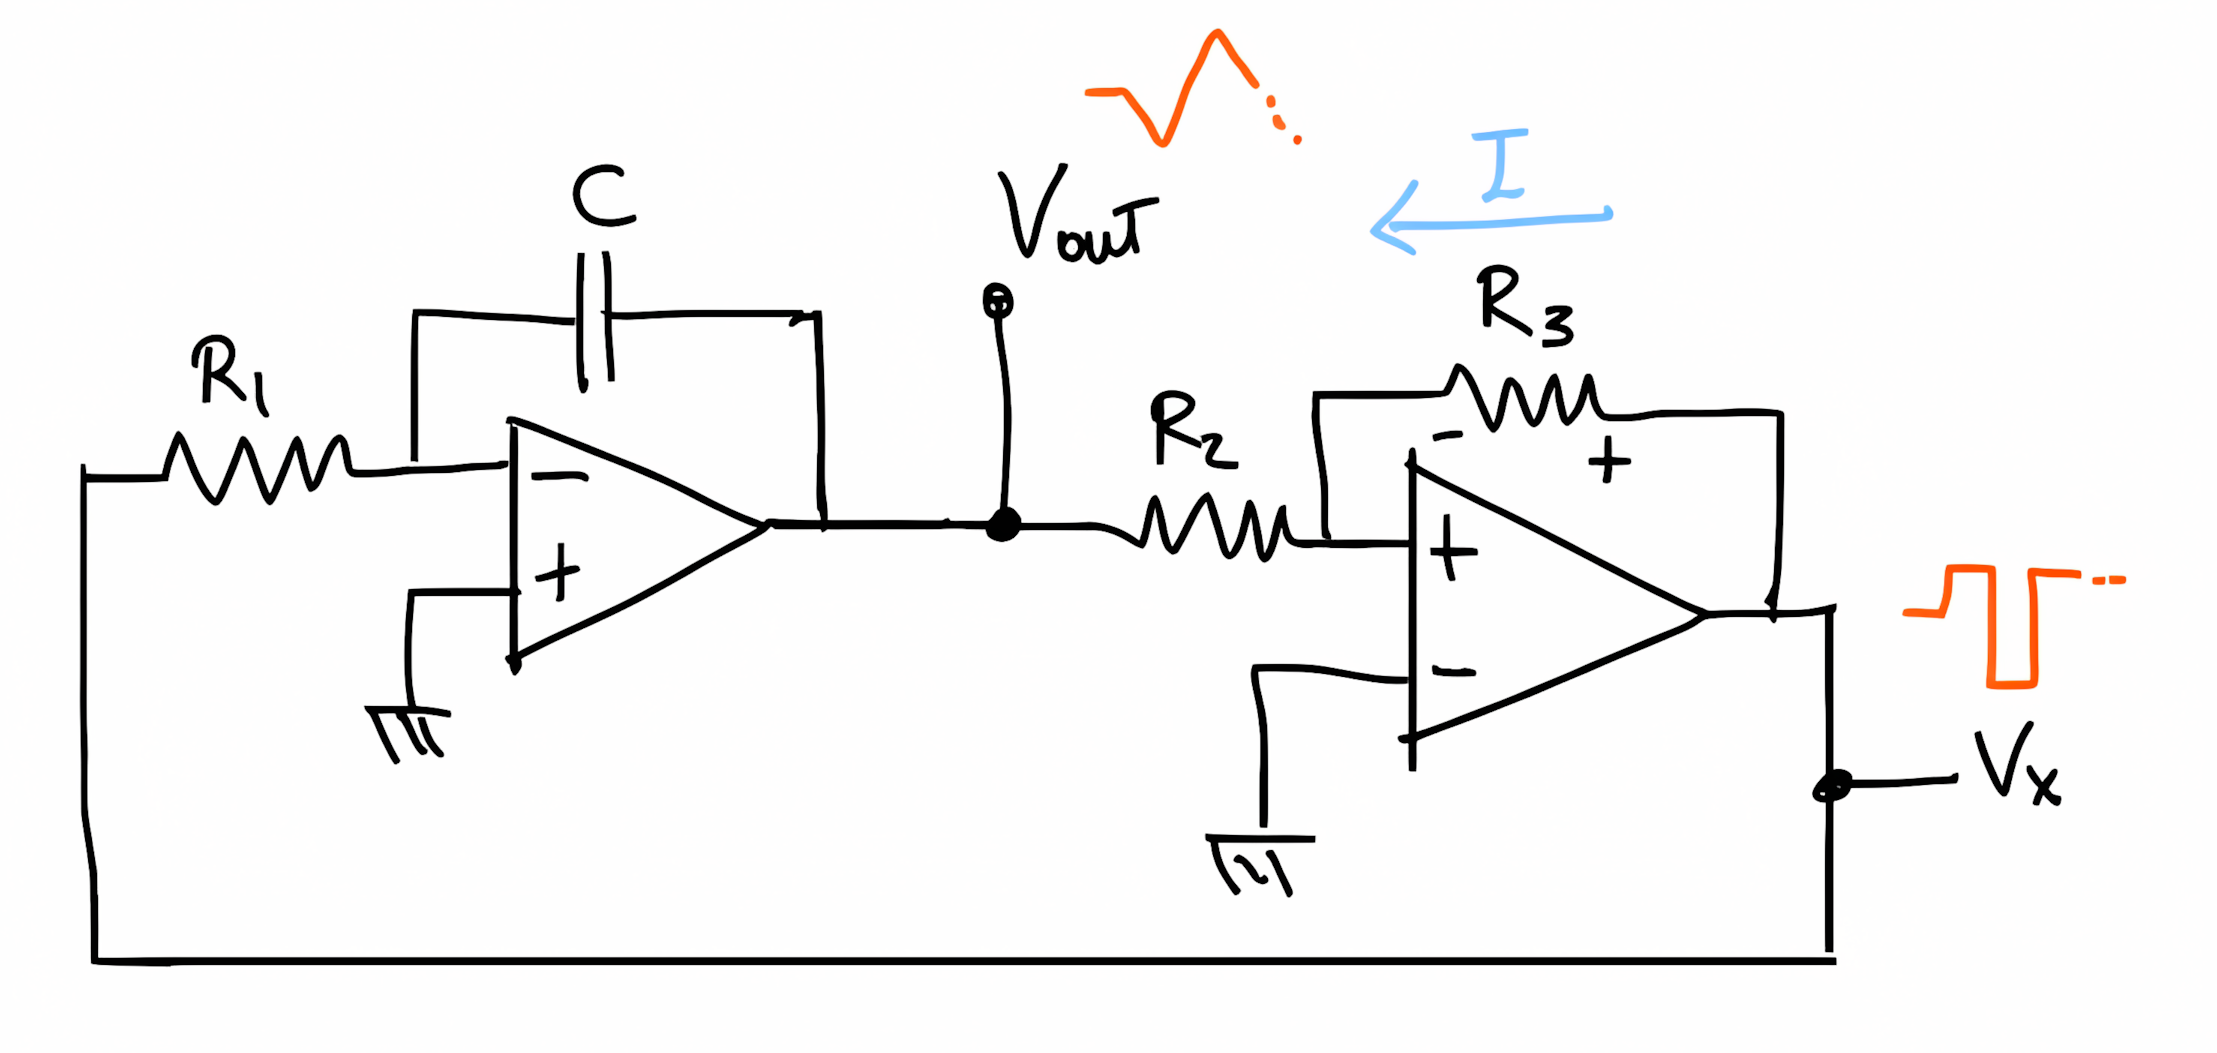
\includegraphics[width=0.6\textwidth]{images/1.6.1.1.png}
    \caption{Generatore di onde triangolari: multivibratore astabile (a destra) e integratore (a sinistra).}
    \label{fig:onda_triangolare}
\end{figure}

Per l’integratore ideale, il cortocircuito virtuale determina una caduta \(L^+\) su \(R_1\), che induce una corrente:
\[
I = \frac{L^+}{R_1}.
\]
Questa corrente carica il condensatore \(C\), la cui tensione è:
\[
V_C = \frac{1}{C}\int \frac{L^+}{R_1}\, dt = \frac{L^+}{R_1C}\, t.
\]
Pertanto, l’uscita dell’integratore è:
\[
V_{\text{out}} = -V_C,
\]
ossia decresce linearmente. Quando \(V_{\text{out}}\) raggiunge il valore di soglia \(V_{TL}\) (determinato dall’analisi del partitore di tensione nella rete astabile), l’output passa a \(L^-\) e il condensatore inizia a scaricarsi verso \(L^-\), facendo variare \(V_{\text{out}}\) in senso opposto. L’alternanza tra \(L^+\) e \(L^-\) genera onde quadre che, integrate, assumono forma triangolare.

\newpage
\subsection{Generatore d’onda quadra}

Consideriamo il circuito in Figura~\ref{fig:onda_quad}, costituito da un multivibratore (A.O. con controreazione positiva) in cui il terminale negativo è collegato a massa tramite un condensatore \(C\) e a \(V_{\text{out}}\) tramite una resistenza \(R_3\).\\[2mm]
\begin{figure}[H]
    \centering
    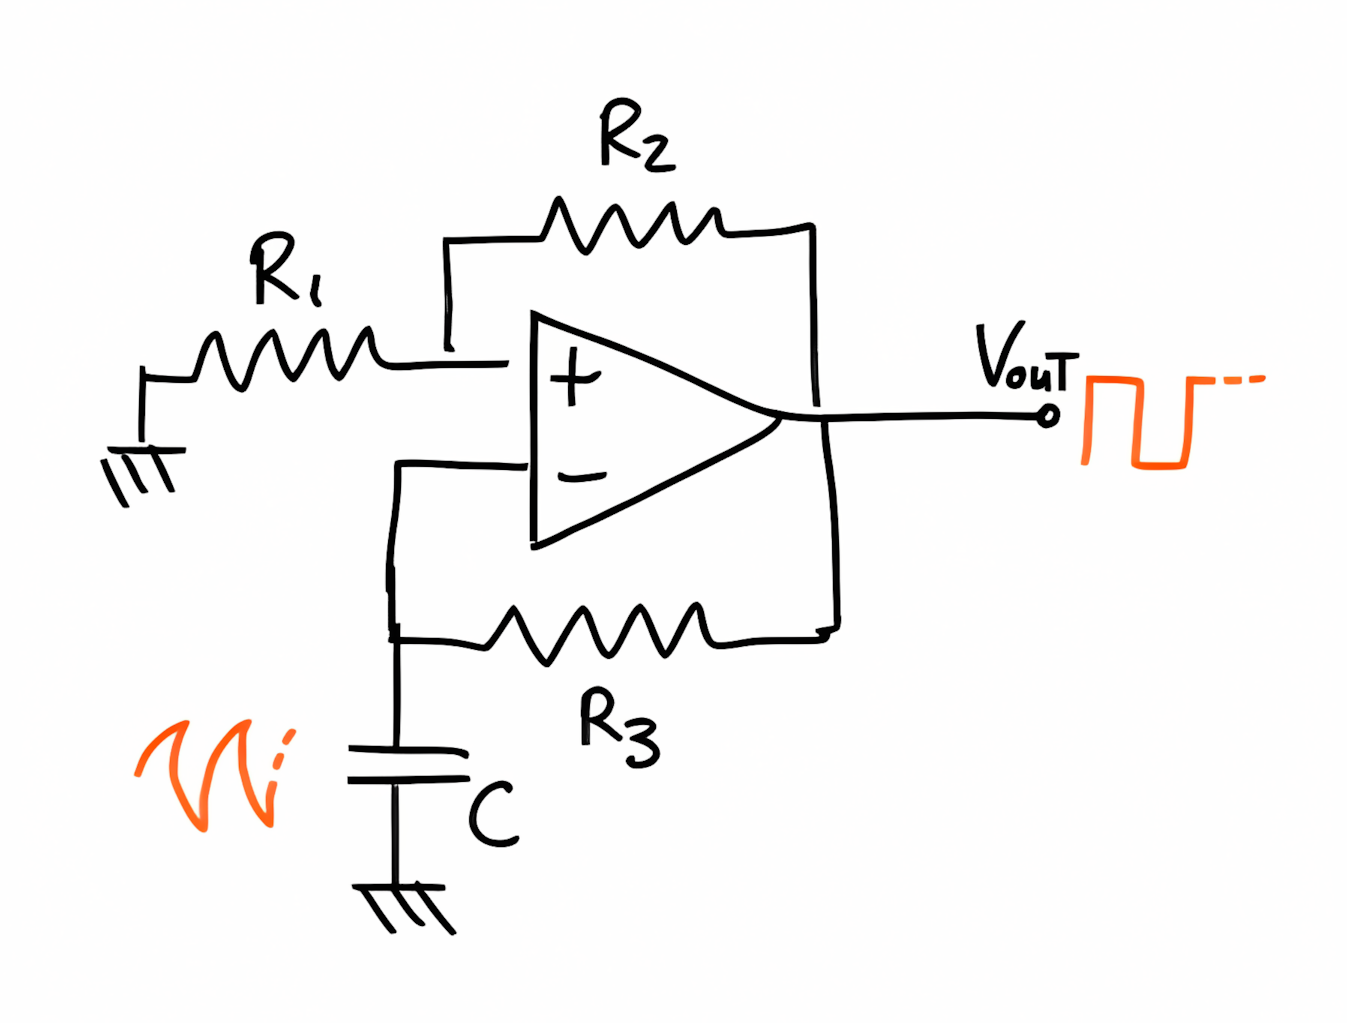
\includegraphics[width=0.6\textwidth]{images/1.6.2.1.png}
    \caption{Circuito di un astabile generatore d’onda quadra.}
    \label{fig:onda_quad}
\end{figure}

Inizialmente, ponendo \(V_{\text{out}} = L^+\), una corrente fluisce da \(V_{\text{out}}\) a massa passando per \(R_2\) e \(R_1\), formando un partitore che definisce:
\[
V^+ = \frac{R_1}{R_1+R_2}\, V_{\text{out}} = \beta\, V_{\text{out}},
\]
con \(\beta = \frac{R_1}{R_1+R_2}\). Il condensatore \(C\) si carica attraverso \(R_3\); quando la tensione \(V_C(t)\) raggiunge \( \beta\, L^+\) (cioè quando \(V^+ - V_C < 0\)), l’A.O. cambia stato e l’output passa a \(L^-\). Il ciclo si ripete, generando un’onda quadra di periodo \(T\).\\[2mm]
\begin{figure}[H]
    \centering
    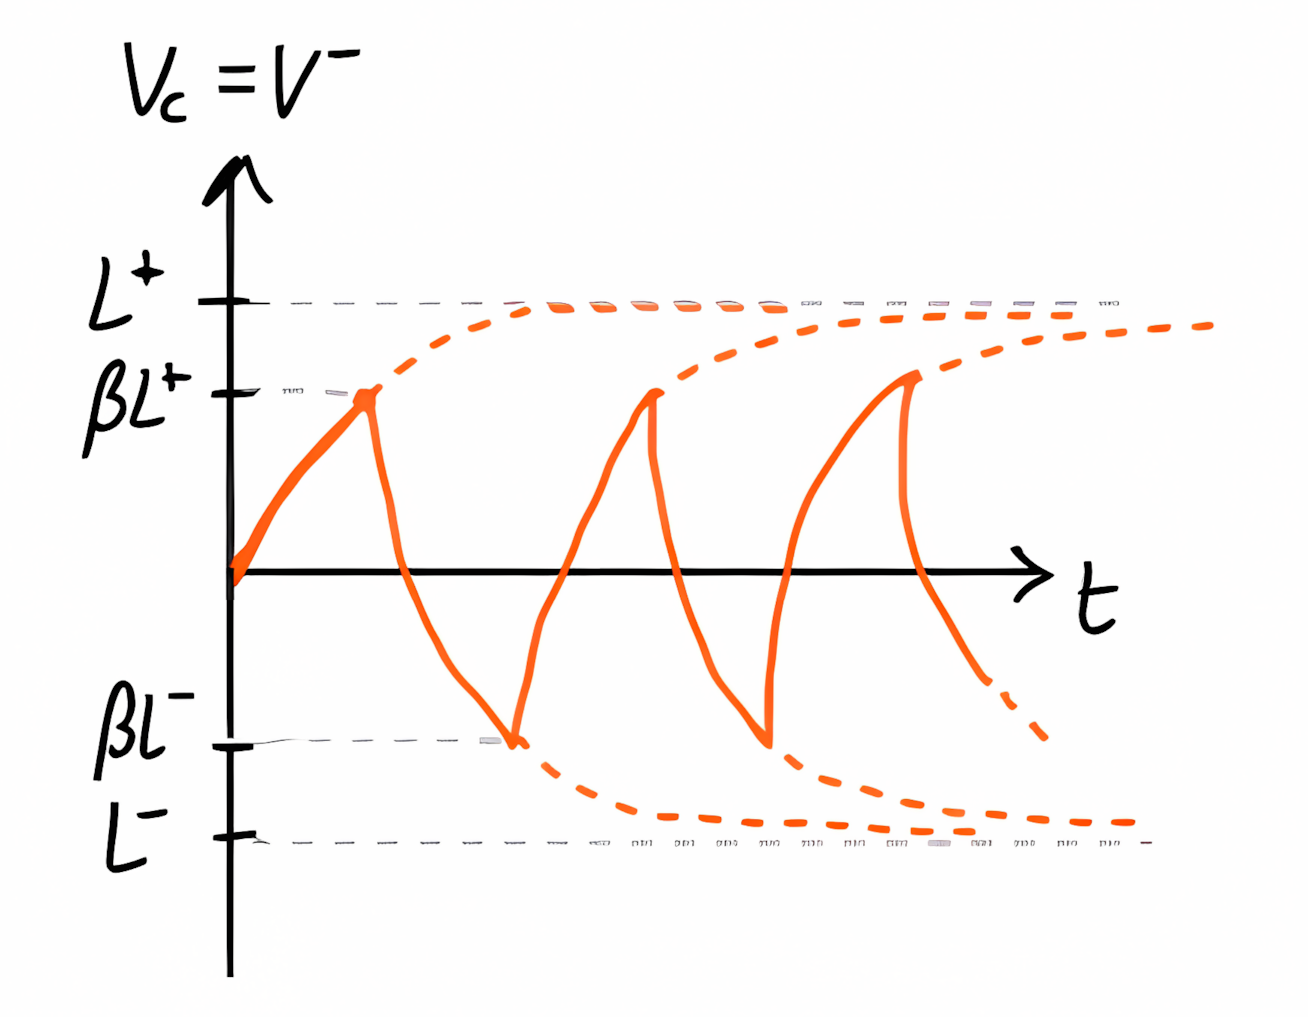
\includegraphics[width=0.6\textwidth]{images/1.6.2.2.png}
    \caption{Andamento temporale della tensione ai capi del condensatore nel generatore d’onda quadra.}
    \label{fig:onda_quad_temp}
\end{figure}
\newpage

\subsection{Trigger di Schmitt Invertente}

Consideriamo lo schema in cui l'amplificatore operazionale è polarizzato mediante retroazione positiva, mentre il segnale d'ingresso viene applicato in configurazione invertente. La struttura circuitale essenziale è illustrata in Figura~\ref{fig:schmitt_invertente}.\\[2mm]
\begin{figure}[H]
  \centering
  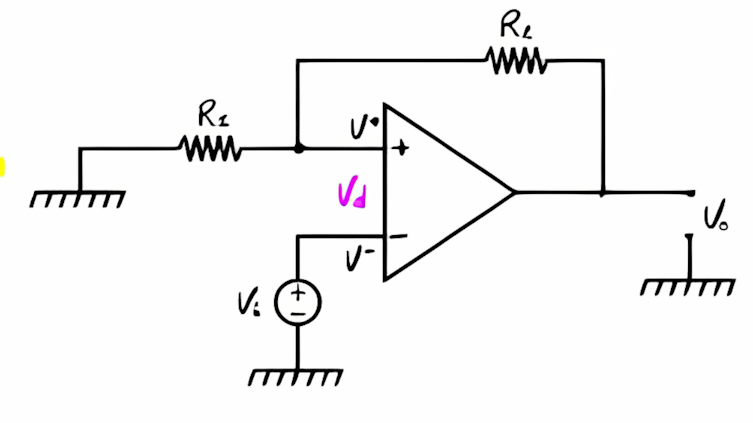
\includegraphics[width=0.48\textwidth]{images/1.6.3.1.png}
  \caption{Schema di principio di un trigger di Schmitt invertente con op-amp.}
  \label{fig:schmitt_invertente}
\end{figure}

Quando l'uscita dell'operazionale satura al livello positivo \(L^+\), il morsetto non invertente assume una tensione data da
\[
V^+ = \beta\, L^+,
\]
dove il coefficiente di divisione
\[
\beta = \frac{R_1}{R_1 + R_2}
\]
è determinato dal partitore formato dai resistori \( R_1 \) e \( R_2 \). In questa condizione, il circuito rimane in saturazione positiva finché il segnale d’ingresso non scende sufficientemente da innescare la commutazione. Esiste dunque una soglia negativa \(V_{\text{TH}^-}\) che, una volta superata, fa passare l’uscita a \(L^-\). Analogamente, quando l'uscita è in saturazione bassa (\(L^-\)), il morsetto non invertente assume:
\[
V^+ = \beta\, L^-.
\]
Il circuito rimane in tale stato fino a quando il segnale d’ingresso non raggiunge la soglia positiva \(V_{\text{TH}^+}\), facendo commutare l'uscita a \(L^+\).

Si definiscono dunque le due soglie di commutazione come:
\[
V_{\text{TH}^+} = \beta\,L^- \qquad \text{e} \qquad V_{\text{TH}^-} = \beta\,L^+.
\]
\\[2mm]
\begin{figure}[H]
  \centering
  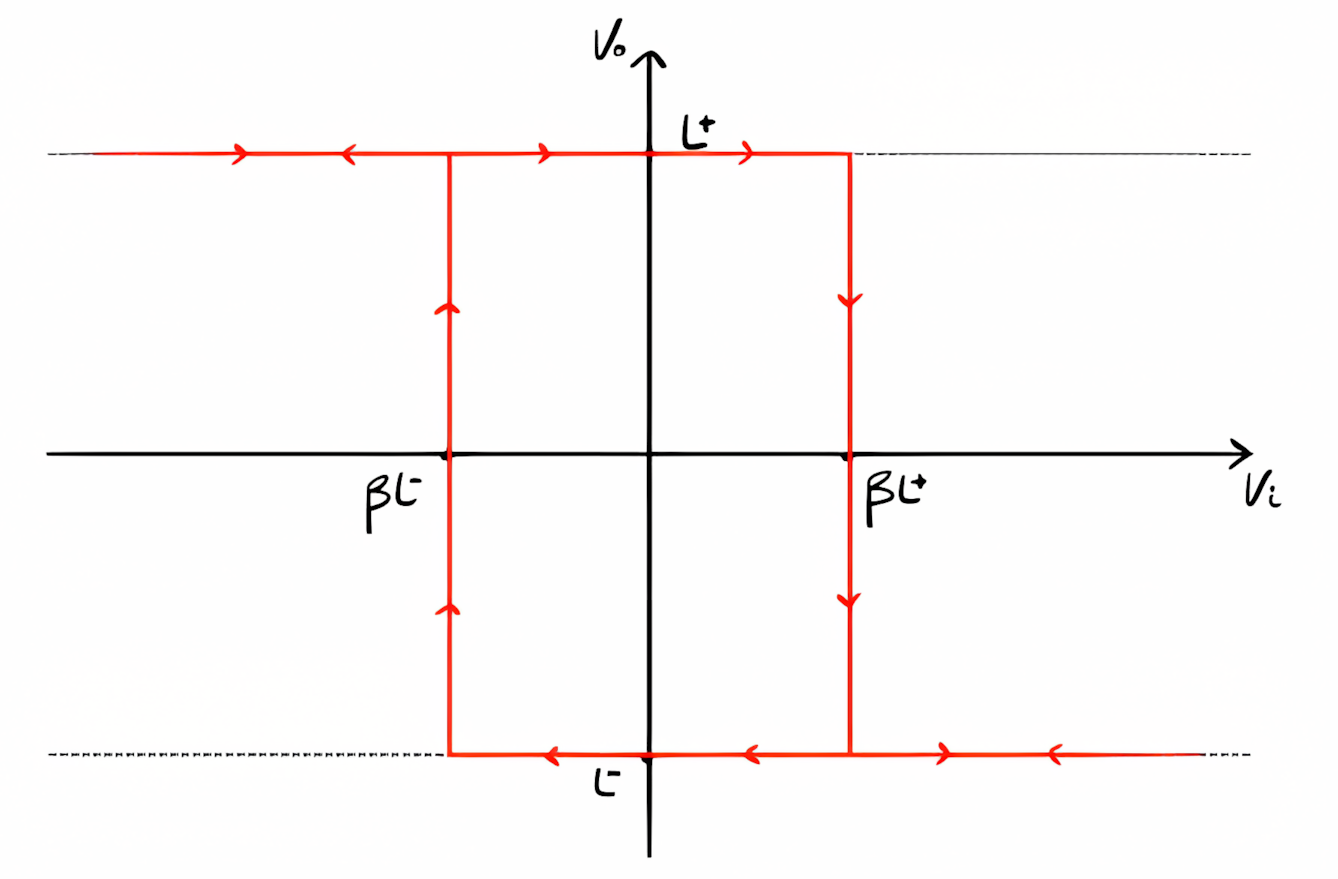
\includegraphics[width=0.48\textwidth]{images/1.6.3.2.png}
  \caption{Funzione di trasferimento del trigger di Schmitt invertente (isteresi).}
  \label{fig:schmitt_invertente_tf}
\end{figure}
\newpage

\subsection{Trigger di Schmitt Non Invertente}

Nel caso del trigger di Schmitt non invertente, il segnale d’ingresso viene applicato al morsetto non invertente dell’operazionale, mentre la retroazione positiva si ottiene collegando l’uscita al medesimo morsetto tramite un partitore di tensione. La configurazione circuitale essenziale è mostrata in Figura~\ref{fig:schmitt_non_invertente}.\\[2mm]
\begin{figure}[H]
  \centering
  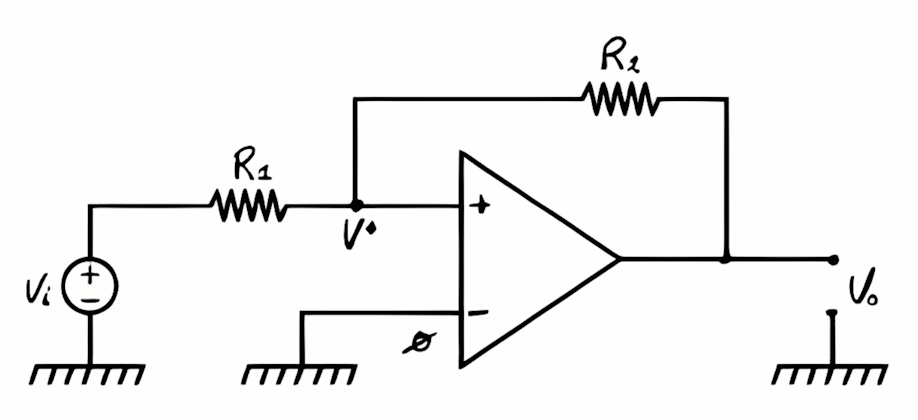
\includegraphics[width=0.45\textwidth]{images/1.6.4.1.png}
  \caption{Schema di principio di un trigger di Schmitt non invertente con op-amp.}
  \label{fig:schmitt_non_invertente}
\end{figure}

Il morsetto invertente viene generalmente mantenuto a un potenziale di riferimento (tipicamente 0\,V). In questa configurazione, la tensione \(V^+\) al morsetto non invertente, ottenuta per sovrapposizione della tensione d’ingresso \(V_{\text{in}}\) e della retroazione, è:
\[
V^{+} = \frac{R_1}{R_1 + R_2}\, V_{\text{out}} + \frac{R_2}{R_1 + R_2}\, V_{\text{in}}.
\]
Quando \(V^{+} > 0\), l’uscita tende a saturare a \(L^+\); viceversa, se \(V^{+} < 0\), l’uscita passa a \(L^-\).

\vspace{2mm}
\textbf{Soglie di commutazione}\\[2mm]
Utilizzando il partitore, si definiscono le soglie:
\[
V_{\text{TH}^+} = \frac{R_1}{R_1 + R_2}\, L^+, \quad V_{\text{TH}^-} = \frac{R_1}{R_1 + R_2}\, L^-.
\]
\\[2mm]
\begin{figure}[H]
  \centering
  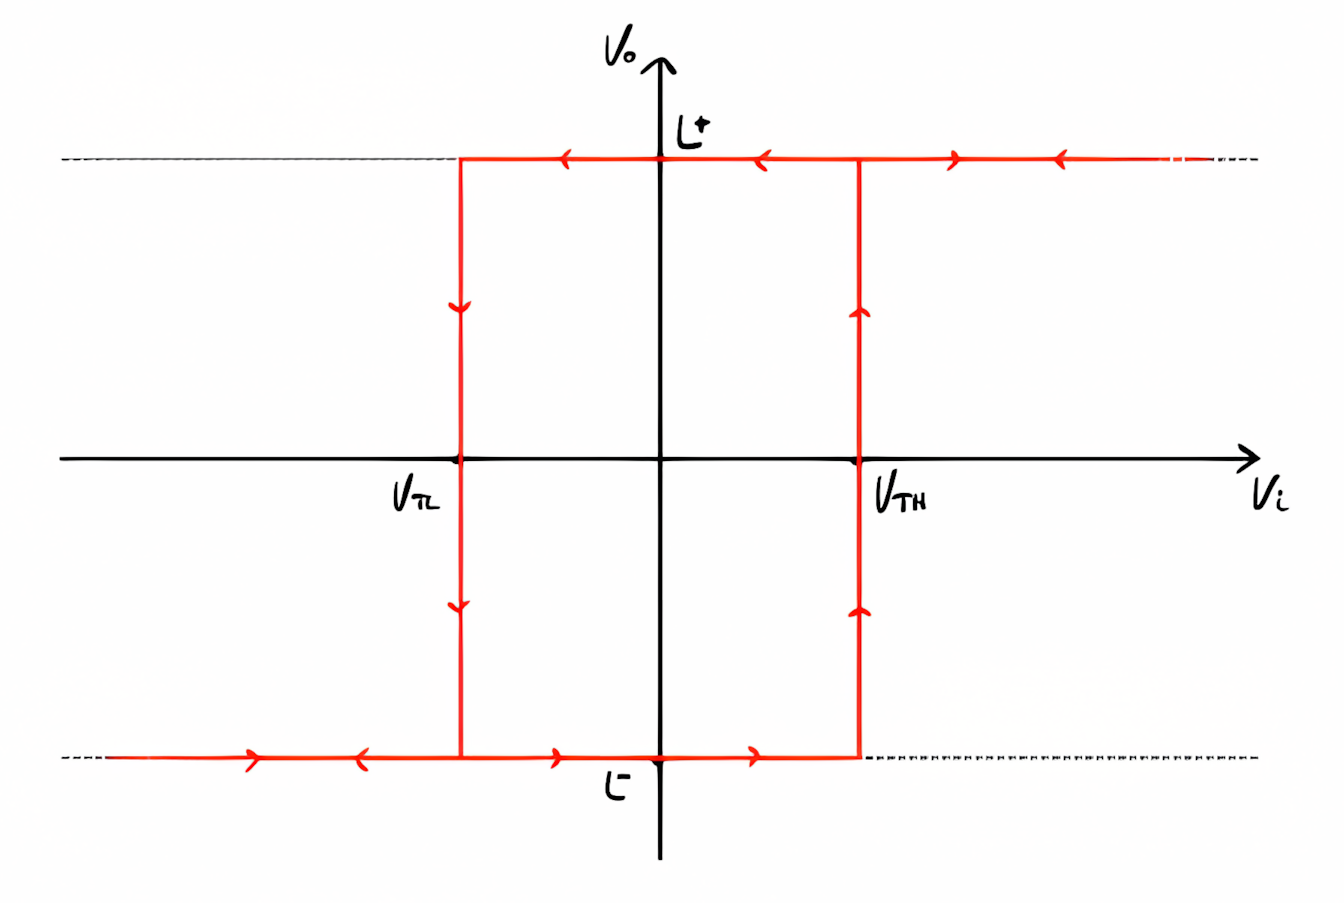
\includegraphics[width=0.45\textwidth]{images/1.6.4.2.png}
  \caption{Funzione di trasferimento del trigger di Schmitt non invertente (isteresi).}
  \label{fig:schmitt_non_invertente_tf}
\end{figure}

